% -*- latex -*-

\chapter{Control Environment}
\label{chap:ControlEnvironment}

\index{control~environment|(}

The control environment is where code interfaces with applications and I/O
devices. The associated API is designed for users that want to use VTK-m to
analyze their data using provided or supplied worklets. Code for the
control environment is designed to run on a single thread (or one single
thread per process in an MPI job).

Most users of VTK-m will have some interaction with the control
environment, for you cannot define data structures or execute any
algorithms without it.

\section{Device Adapter Tag}
\label{sec:DeviceAdapterTag}

\index{device~adapter|(}

VTK-m uses a feature called a device adapter to define what type of device
will be used to run algorithms. The device adapter encapsulates the
device-specific code required to port to various devices. More information
on the function of the device adapter is given in
Section~\ref{sec:DeviceIndependence}.
% Link from original Dax document. Need to find a place for it.

The device adapter is identified by a \keyterm{device adapter tag}.
\index{device~adapter~tag} \index{tag!device~adapter} This tag, which is
simply an empty struct type, is used as the template parameter for several
classes in the VTK-m control environment and causes these classes to direct
their work to a particular device.

There are two ways to select a device adapter. The first is to make a
global selection of a default device adapter. The second is to specify a
specific device adapter as a template parameter.

\subsection{Default Device Adapter}

A default device adapter tag is specified in
\vtkmheader{vtkm/cont}{DeviceAdapter.h} (although it can also by specified
in many other VTK-m headers via header dependencies). If no other
information is given, VTK-m attempts to choose a default device adapter
that is a best fit for the system it is compiled on. VTK-m currently select
the default device adapter with the following sequence of conditions.

\begin{itemize}
\item \index{CUDA} If the source code is being compiled by CUDA, the CUDA
  device is used.
\item \index{OpenMP} If the CUDA compiler is not being used and the current
  compiler supports OpenMP, then the OpenMP device is used.
  \fix{Technically, OpenMP is not yet supported in VTK-m, so this will
    never actually be picked. But once it is implemented, this will be the
    chain.}
\item \index{Intel Threading Building Blocks} \index{TBB} If the compiler
  supports neither CUDA nor OpenMP and VTK-m was configured to use Intel
  Threading Building Blocks, then that device is used.
\item \index{serial} If no parallel device adapters are found, then VTK-m
  falls back to a serial device.
\end{itemize}

You can also set the default device adapter specifically by setting the
\vtkmmacro{VTKM\_DEVICE\_ADAPTER} macro. This macro must be set
\emph{before} including any VTK-m files. You can set
\vtkmmacro{VTKM\_DEVICE\_ADAPTER} to any one of the following.

\begin{description}
\item[\vtkmmacro{VTKM\_DEVICE\_ADAPTER\_SERIAL}] Performs all computation on
  the same single thread as the control environment. This device is useful
  for debugging. This device is always available.
\item[\vtkmmacro{VTKM\_DEVICE\_ADAPTER\_CUDA}] Uses a CUDA capable GPU
  device. For this device to work, VTK-m must be configured to use CUDA and
  the code must be compiled by the CUDA \textfilename{nvcc} compiler.
\item[\vtkmmacro{VTKM\_DEVICE\_ADAPTER\_OPENMP}] Uses OpenMP compiler
  extensions to run algorithms on multiple threads. For this device to
  work, VTK-m must be configured to use OpenMP and the code must be
  compiled with a compiler that supports OpenMP pragmas. \fix{Not currently
    implemented.}
\item[\vtkmmacro{VTKM\_DEVICE\_ADAPTER\_TBB}] Uses the Intel Threading
  Building Blocks library to run algorithms on multiple threads. For this
  device to work, VTK-m must be configured to use TBB and the executable
  must be linked to the TBB library.
\end{description}

These macros provide a useful mechanism for quickly reconfiguring code to
run on different devices. The following example shows a typical block of
code at the top of a source file that could be used for quick
reconfigurations.

\vtkmlisting{Macros to port VTK-m code among different devices}{DefaultDeviceAdapter.cxx}

The default device adapter can always be overridden by specifying a device
adapter tag, as described in the next section. There is actually one more
internal default device adapter named
\vtkmmacro{VTKM\_DEVICE\_ADAPTER\_ERROR} that will cause a compile error if
any component attempts to use the default device adapter. This feature is
most often used in testing code to check when device adapters should be
specified.

\subsection{Specifying Device Adapter Tags}

In addition to setting a global default device adapter, it is possible to
explicitly set which device adapter to use in any feature provided by
VTK-m. This is done by providing a device adapter tag as a template
argument to VTK-m templated objects. The following device adapter tags are
available in VTK-m.

\index{device~adapter~tag|(}
\index{tag!device~adapter|(}

\begin{description}
\item[\vtkmcont{DeviceAdapterTagSerial}] \index{serial} Performs all
  computation on the same single thread as the control environment. This
  device is useful for debugging. This device is always available. This tag
  is defined in \vtkmheader{vtkm/cont}{DeviceAdapterSerial.h}.
\item[\vtkmcont{DeviceAdapterTagCuda}] \index{CUDA} Uses a CUDA capable
  GPU device. For this device to work, VTK-m must be configured to use CUDA
  and the code must be compiled by the CUDA \textfilename{nvcc}
  compiler. This tag is defined in
  \vtkmheader{vtkm/cont/cuda}{DeviceAdapterCuda.h}.
\item[\vtkmcont{DeviceAdapterTagOpenMP}] \index{OpenMP} Uses OpenMP
  compiler extensions to run algorithms on multiple threads. For this
  device to work, VTK-m must be configured to use OpenMP and the code must be
  compiled with a compiler that supports OpenMP pragmas. This tag is
  defined in \vtkmheader{vtkm/openmp/cont}{DeviceAdapterOpenMP.h}. \fix{Not
    currently implemented.}
\item[\vtkmcont{DeviceAdapterTagTBB}]
  \index{Intel Threading Building Blocks} \index{TBB} Uses the Intel
  Threading Building Blocks library to run algorithms on multiple
  threads. For this device to work, VTK-m must be configured to use TBB and
  the executable must be linked to the TBB library. This tag is defined in
  \vtkmheader{vtkm/cont/tbb}{DeviceAdapterTBB.h}.
\end{description}

\fix{Add example. I would like to have a simple example involving a filter,
but that interface is still in flux.}
%% The following example invokes the elevation worklet much like shown in
%% Example~\ref{ex:Elevation} on page~\pageref{ex:Elevation} but also
%% specifies using the Intel Threading Building blocks device adapter.
%% \index{Intel Threading Building Blocks} \index{TBB}
%% In particular, consider the template parameter of the
%% \daxcont{DispatcherMapField} class.
%% \begin{daxexample}{Calling the Elevation worklet with a specific device adapter.}
%% dax::worklet::Elevation elevation(dax::make_Vector3(-1.0, 0.0, 0.0),
%%                                   dax::make_Vector3(1.0, 0.0, 0.0),
%%                                   dax::make_Vector2(-1.0, 1.0));

%% dax::cont::DispatcherMapField<dax::worklet::Elevation, dax::tbb::cont::DeviceAdapterTagTBB>
%%     dispatcher(elevation);
%% dispatcher.Invoke(grid.GetPointCoordinates(), outPointElevation);
%% \end{daxexample}

When structuring your code to always specify a particular device adapter,
consider setting the default device adapter (with the
\vtkmmacro{VTKM\_DEVICE\_ADAPTER} macro) to
\vtkmmacro{VTKM\_DEVICE\_ADAPTER\_ERROR}. This will cause the compiler to
produce an error if any object is instantiated with the default device
adapter, which checks to make sure the code properly specifies every device
adapter parameter.

VTK-m also defines a macro named
\vtkmmacro{VTKM\_DEFAULT\_DEVICE\_ADAPTER\_TAG}, which can be used in place
of an explicit device adapter tag to use the default tag. This macro is
used to create new templates that have template parameters for device
adapters that can use the default. The following example has a (rather
artificial) declaration of a helper class for executing the elevation
filter.

\fix{Add example when filters are settled.}

%% \begin{daxexample}{Declaring a template with a default device adapter.}
%% template<typename DeviceAdapter = DAX_DEFAULT_DEVICE_ADAPTER_TAG>
%% class MyElevationDispatcher
%% {
%% public:
%%   void DoInvoke()
%%   {
%%     dax::cont::DispatcherMapField<dax::Worklet::Elevation,DeviceAdapter> dispatcher;
%%     dispatcher.Invoke(this->Grid.GetPointCoordinates(), this->OutPointElevation);
%% \end{daxexample}

\index{tag!device~adapter|)}
\index{device~adapter~tag|)}

\index{device~adapter|)}

\section{Array Handle}
\label{sec:ArrayHandle}

\index{array~handle|(}

An \keyterm{array handle}, implemented with the \vtkmcont{ArrayHandle}
class, manages an array of data that can be accessed or manipulated by VTK-m
algorithms. It is typical to construct an array handle in the control
environment to pass data to an algorithm running in the execution
environment. It is also typical for an algorithm running in the execution
environment to allocate and populate an array handle, which can then be
read back in the control environment. It is also possible for an array
handle to manage data created by one VTK-m algorithm and passed to another,
remaining in the execution environment the whole time and never copied to
the control environment.

The array handle may have up to two copies of the array, one for the
control environment and one for the execution environment. However,
depending on the device and how the array is being used, the array handle
will only have one copy when possible. Copies between the environments are
implicit and lazy. They are copied only when an operation needs data in an
environment where the data is not.

\vtkmcont{ArrayHandle} behaves like a shared smart pointer in that when the
C++ object is copied, each copy holds a reference to the same array. These
copies are reference counted so that when all copies of the
\vtkmcont{ArrayHandle} are destroyed, any allocated memory is released.

\subsection{Creating Array Handles}

\vtkmcont{ArrayHandle} is a templated class with two template
parameters. The first template parameter is the only one required and
specifies the base type of the entries in the array. The second template
parameter specifies the storage used when storing data in the control
environment. Storage objects are discussed later in this section, and for
now we will use the default value.

\begin{vtkmexample}{Declaration of the \protect\vtkmcont{ArrayHandle} templated class.}
template<
    typename T,
    typename StorageTag = VTKM_DEFAULT_STORAGE_TAG>
class ArrayHandle;
\end{vtkmexample}

There are multiple ways to create and populate an array handle. The default
\vtkmcont{ArrayHandle} constructor will create an empty array with nothing
allocated in either the control or execution environment. This is
convenient for creating arrays used as the output for algorithms.

\vtkmlisting{Creating an \textidentifier{ArrayHandle} for output data.}{CreateArrayHandle.cxx}

Constructing an \vtkmcont{ArrayHandle} that points to a provided C array or
\textcode{std::vector} is straightforward with the
\vtkmcont{make\_ArrayHandle} functions. These functions will make an array
handle that points to the array data that you provide.

\vtkmlisting{Creating an \textidentifier{ArrayHandle} that points to a provided C array.}{ArrayHandleFromCArray.cxx}

\vtkmlisting[ex:ArrayHandleFromVector]{Creating an \textidentifier{ArrayHandle} that points to a provided \textcode{std::vector}.}{ArrayHandleFromVector.cxx}

\emph{Be aware} that \vtkmcont{make\_ArrayHandle} makes a shallow pointer
copy. This means that if you change or delete the data provided, the
internal state of \vtkmcont{ArrayHandle} becomes invalid and undefined
behavior can ensue. The most common manifestation of this error happens
when a \textcode{std::vector} goes out of scope. This subtle interaction
will cause the \vtkmcont{ArrayHandle} to point to an unallocated portion of
the memory heap. For example, if the code in
Example~\ref{ex:ArrayHandleFromVector} where to be placed within a callable
function or method, it could cause the \vtkmcont{ArrayHandle} to become
invalid.

\vtkmlisting{Invalidating an \textidentifier{ArrayHandle} by letting the source \textcode{std::vector} leave scope.}{ArrayOutOfScope.cxx}

\subsection{Array Portals}
\label{sec:ArrayPortals}

\index{array~portal|(}

An array handle defines auxiliary structures called \keyterm{array portals}
that provide direct access into its data. An array portal is a simple
object that is somewhat functionally equivalent to an STL-type iterator, but
with a much simpler interface. Array portals can be read-only (const) or
read-write and they can be accessible from either the control environment
or the execution environment. All these variants have similar interfaces
although some features that are not applicable can be left out.

An array portal object contains each of the following:
\begin{description}
\item[\textcode{ValueType}] A \textcode{typedef} of the type for each item
  in the array.
\item[\textcode{GetNumberOfValues}] A method that returns the number of
  entries in the array.
\item[\textcode{Get}] A method that returns the value at a given index.
\item[\textcode{Set}] A method that changes the value at a given
  index. This method does not need to exist for read-only (const) array
  portals.
\end{description}

The following code example defines an array portal for a simple C array of
scalar values. This definition has no practical value (it is covered by the
more general \vtkmcontinternal{ArrayPortalFromIterators}), but demonstrates
the function of each component.

\vtkmlisting{A simple array portal implementation.}{SimpleArrayPortal.cxx}

Although array portals are simple to implement and use, and array portals'
functionality is similar to iterators, there exists a great deal of code
already based on STL iterators and it is often convienient to interface
with an array through an iterator rather than an array portal. The
\vtkmcont{ArrayPortalToIterators} class can be used to convert an array
portal to an STL-compatible iterator. The class is templated on the array
portal type and has a constructor that accepts an instance of the array
portal. It contains the following features.
\begin{description}
\item[\textcode{IteratorType}] A \textcode{typedef} of an STL-compatible
  random-access iterator that can provide the same access as the array
  portal.
\item[\textcode{GetBegin}] A method that returns an STL-compatible iterator
  of type \textcode{IteratorType} that points to the beginning of the
  array.
\item[\textcode{GetEnd}] A method that returns an STL-compatible iterator
  of type \textcode{IteratorType} that points to the end of the array.
\end{description}

\vtkmlisting{Using \textidentifier{ArrayPortalToIterators}.}{ArrayPortalToIterators.cxx}

As a convenience, \vtkmheader{vtkm/cont}{ArrayPortalToIterators.h} also
defines a pair of functions named \textcode{ArrayPortalToIteratorBegin}
\index{ArrayPortalToIteratorBegin} and \textcode{ArrayPortalToIteratorEnd}
\index{ArrayPortalToIteratorEnd} that each take an array portal as an
argument and return a begin and end iterator, respectively.

\vtkmlisting{Using \textidentifier{ArrayPortalToIteratorBegin} and \textidentifier{ArrayPortalToIteratorEnd}.}{ArrayPortalToIteratorBeginEnd.cxx}

\vtkmcont{ArrayHandle} contains two \textcode{typedef}s for array portal
types that are capable of interfacing with the underlying data in the
control environment. These are \textcode{PortalControl}
\index{PortalControl} and \textcode{PortalConstControl},
\index{PortalConstControl} which define read-write and read-only (const)
array portals, respectively.

\vtkmcont{ArrayHandle} also contains similar \textcode{typedef}s for array
portals in the execution environment. Because these types are dependent on
the device adapter used for execution, these typedefs are embedded in a
templated class named \textcode{ExecutionTypes}. \index{ExecutionTypes}
Within \textcode{ExecutionTypes} are the typedefs \textcode{Portal} and
\textcode{PortalConst} defining the read-write and read-only (const) array
portals, respectively, for the execution environment for the given device
adapter tag.

Because \vtkmcont{ArrayHandle} is an control environment object, it
provides the methods \textcode{GetPortalControl} \index{GetPortalControl}
and \textcode{GetPortalConstControl} \index{GetPortalConstControl} to get
the associated array portal objects. These methods also have the side
effect of refreshing the control environment copy of the data, so this can
be a way of synchronizing the data. Be aware that when an
\vtkmcont{ArrayHandle} is created with a pointer or \textcode{std::vector},
it is put in a read-only mode, and \textcode{GetPortalControl} can fail
(although \textcode{GetPortalConstControl} will still work). Also be aware
that calling \textcode{GetPortalControl} will invalidate any copy in the
execution environment, meaning that any subsequent use will cause the data
to be copied back again.

\vtkmlisting{Using portals from an \textidentifier{ArrayHandle}.}{ControlPortals.cxx}

\index{array~portal|)}

\subsection{Interface to Execution Environment}
\label{sec:ArrayHandleInterfaceToExecutionEnvironment}

One of the main functions of the array handle is to allow an array to be
defined in the control environment and then be used in the execution
environment. When using an \textidentifier{ArrayHandle} with worklets
\fix{or filters?}, this transition is handled automatically. However, it is
also possible to invoke the transfer for use in your own scheduled
algorithms.

The \textidentifier{ArrayHandle} class manages the transition from control
to execution with a set of three methods that allocate, transfer, and ready
the data in one operation. These methods all start with the prefix
\textcode{Prepare} and are meant to be called before some operation happens
in the execution environment. The methods are as follows.

\begin{description}
\item[\textcode{PrepareForInput}] \index{PrepareForInput} Copies data from
  the control to the execution environment, if necessary, and readies the
  data for read-only access.
\item[\textcode{PrepareForInPlace}] \index{PrepareForInPlace} Copies the
  data from the control to the execution environment, if necessary, and
  readies the data for both reading and writing.
\item[\textcode{PrepareForOutput}] \index{PrepareForOutput} Allocates space
  (the size of which is given as a parameter) in the execution environment,
  if necessary, and readies the space for writing.
\end{description}

The \textcode{PrepareForInput} and \textcode{PrepareForInPlace} methods
each take a single argument that is the device adapter tag where execution
will take place (see Section~\ref{sec:DeviceAdapterTag} for more
information on device adapter tags). \textcode{PrepareForOutput} takes two
arguments: the size of the space to allocate and the device adapter tag.
Each of these methods returns an array portal that can be used in the
execution environment. \textcode{PrepareForInput} returns an object of type
\textidentifier{ArrayHandle}\textcode{:\colonhyp{}ExecutionTypes<{\it{}DeviceAdapterTag}>:\colonhyp{}PortalConst}
whereas \textcode{PrepareForInPlace} and \textcode{PrepareForOutput} each
return an object of type
\textidentifier{ArrayHandle}\textcode{:\colonhyp{}ExecutionTypes<{\it{}DeviceAdapterTag}>:\colonhyp{}Portal}.

Although these \textcode{Prepare} methods are called in the control
environment, the returned array portal can only be used in the execution
environment. Thus, the portal must be passed to an invocation of the
execution environment. Typically this is done with a call to
\textcode{Schedule} in \vtkmcont{DeviceAdapterAlgorithm}. This and other
device adapter algorithms are described in detail in
Section~\ref{sec:DeviceAdapterAlgorithms}, but here is a quick example of
using these execution array portals in a simple functor.

\vtkmlisting{Using an execution array portal from an \textidentifier{ArrayHandle}.}{ExecutionPortals.cxx}

It should be noted that the array handle will expect any use of the
execution array portal to finish before the next call to any
\textidentifier{ArrayHandle} method. Since these \textcode{Prepare} methods
are typically used in the process of scheduling an algorithm in the
execution environment, this is seldom an issue.

\subsection{Basic Storage}

\index{array~handle!storage|(}
\index{storage|(}

As previously discussed, \vtkmcont{ArrayHandle} takes two template arguments.
\begin{vtkmexample}{Declaration of the \protect\vtkmcont{ArrayHandle} templated class (again).}
template<
    typename T,
    typename StorageTag = VTKM_DEFAULT_STORAGE_TAG>
class ArrayHandle;
\end{vtkmexample}
The first argument is the only one required and has been demonstrated
multiple times before. The second (optional) argument specifies something
called a storage, which provides the interface between the generic
\vtkmcont{ArrayHandle} class and a specific storage mechanism in the
control environment.

In this and the following sections we describe this storage mechanism.  A
default storage is specified in much the same way as a default device
adapter is defined. It is done by setting the \vtkmmacro{VTKM\_STORAGE}
macro. This macro must be set before including any VTK-m header
files. Currently the only practical storage provided by VTK-m is the basic
storage, which simply allocates a continuous section of memory of the given
base type. This storage can be explicitly specified by setting
\vtkmmacro{VTKM\_STORAGE} to \vtkmmacro{VTKM\_STORAGE\_BASIC} although the
basic storage will also be used as the default if no other storage is
specified (which is typical).

The default storage can always be overridden by specifying an array
storage tag. The tag for the basic storage is located in the
\vtkmheader{vtkm/cont}{StorageBasic.h} header file and is named
\vtkmcont{StorageTagBasic}. Here is an example of specifying
the storage type when declaring an array handle.

\vtkmlisting{Specifying the storage type for an \textidentifier{ArrayHandle.}}{ArrayHandleStorageParameter.cxx}

VTK-m also defines a macro named \vtkmmacro{VTKM\_DEFAULT\_STORAGE\_TAG}
that can be used in place of an explicit storage tag to use the
default tag. This macro is used to create new templates that have template
parameters for storage that can use the default.

\subsection{Adapting Data Structures}

\index{array~handle!adapting|(}
\index{storage!adapting|(}

The intention of the storage parameter for \vtkmcont{ArrayHandle} is to
implement the strategy design pattern to enable VTK-m to interface directly
with the data of any third party code source. VTK-m is designed to work
with data originating in other libraries or applications. By creating a new
type of storage, VTK-m can be entirely adapted to new kinds of data
structures.

In this section we demonstrate the steps required to adapt the array handle
to a data structure provided by a third party. For the purposes of the
example, let us say that some fictitious library named ``foo'' has a simple
structure named \textcode{FooFields} that holds the field values for a
particular part of a mesh, and then maintain the field values for all
locations in a mesh in a \textcode{std::deque} object.

\vtkmlisting{Fictitious field storage used in custom array storage examples.}{FictitiousFieldStorage.cxx}

VTK-m expects separate arrays for each of the fields rather than a single
array containing a structure holding all of the fields. However, rather
than copy each field to its own array, we can create a storage for each
field that points directly to the data in a \textcode{FooFieldsDeque}
object.

The first step in creating an adapter storage is to create a control
environment array portal to the data. This is described in more detail in
Section~\ref{sec:ArrayPortals} and is generally straightforward for simple
containers like this. Here is an example implementation for our
\textcode{FooFieldsDeque} container.

\vtkmlisting[ex:ArrayPortalAdapter]{Array portal to adapt a third-party container to VTK-m.}{ArrayPortalAdapter.cxx}

The next step in creating an adapter storage is to define a tag for the
adapter. We shall call ours
\textcode{StorageTagFooPressure}. Then, we need to create a
specialization of the templated \vtkmcontinternal{Storage}
class. The \textidentifier{ArrayHandle} will instantiate an object using
the array container tag we give it, and we define our own specialization so
that it runs our interface into the code.

\vtkmcontinternal{Storage} has two template arguments: the
base type of the array and the storage tag.

\vtkmlisting{Prototype for \protect\vtkmcontinternal{Storage}.}{StoragePrototype.cxx}

The \vtkmcontinternal{Storage} must define the following items.
\begin{description}
\item[\textcode{ValueType}] A \textcode{typedef} of the type for each item
  in the array. This is the same type as the first template argument.
\item[\textcode{PortalType}] The type of an array portal that can be used
  to access the underlying data. This array portal needs to work only in
  the control environment.
\item[\textcode{PortalConstType}] A read-only (const) version of
  \textcode{PortalType}.
\item[\textcode{GetPortal}] A method that returns an array portal of type
  \textcode{PortalType} that can be used to access the data manged in this
  storage.
\item[\textcode{GetPortalConst}] Same as \textcode{GetPortal} except it
  returns a read-only (const) array portal.
\item[\textcode{GetNumberOfValues}] A method that returns the number of
  values the storage is currently allocated for.
\item[\textcode{Allocate}] A method that allocates the array to a given
  size. An values stored in the previous allocation may be destroyed.
\item[\textcode{Shrink}] A method like \textcode{Allocate} with two
  differences. First, the size of the allocation must be smaller than the
  existing allocation when the method is called. Second, any values
  currently stored in the array will be valid after the array is
  resized. This constrained form of allocation allows the array to be
  resized and values valid without ever having to copy data.
\item[\textcode{ReleaseResources}] A method that instructs the storage to
  free all of its memory.
\end{description}

The following provides an example implementation of our adapter to a
\textcode{FooFieldsDeque}. It relies on the
\textcode{ArrayPortalFooPressure} provided in
Example~\ref{ex:ArrayPortalAdapter}.

\vtkmlisting{Storage to adapt a third-party container to VTK-m.}{StorageAdapter.cxx}

\index{array~handle!subclassing}

The final step to make a storage adapter is to make a mechanism to
construct an \textidentifier{ArrayHandle} that points to a particular
storage. This can be done by creating a trivial subclass of
\vtkmcont{ArrayHandle} that simply constructs the array handle to the state
of an existing container.

\vtkmlisting[ex:ArrayHandleAdapter]{Array handle to adapt a third-party container to VTK-m.}{ArrayHandleAdapter.cxx}

\label{sec:VTKM_ARRAY_HANDLE_SUBCLASS_NT}

Subclasses of \textidentifier{ArrayHandle} provide constructors that
establish the state of the array handle. All array handle subclasses must
also use either the \vtkmmacro{VTKM\_ARRAY\_HANDLE\_SUBCLASS} macro or the
\vtkmmacro{VTKM\_ARRAY\_HANDLE\_SUBCLASS\_NT} macro. Both of these macros
define the typedefs \textcode{Superclass}, \textcode{ValueType}, and
\textcode{StorageTag} as well as a set of constructors and operators
expected of all \textidentifier{ArrayHandle} classes. The difference
between these two macros is that \vtkmmacro{VTKM\_ARRAY\_HANDLE\_SUBCLASS}
is used in templated classes whereas
\vtkmmacro{VTKM\_ARRAY\_HANDLE\_SUBCLASS\_NT} is used in non-templated
classes.

The \textidentifier{ArrayHandle} subclass in
Example~\ref{ex:ArrayHandleAdapter} is not templated, so it uses
the \vtkmmacro{VTKM\_ARRAY\_HANDLE\_SUBCLASS\_NT} macro. (The other macro
is described in Section~\ref{sec:VTKM_ARRAY_HANDLE_SUBCLASS} on
page~\pageref{sec:VTKM_ARRAY_HANDLE_SUBCLASS}). This macro takes two
parameters. The first parameter is the name of the subclass where the macro
is defined and the second parameter is the immediate superclass including
the full template specification. The second parameter of the macro must be
enclosed in parentheses so that the C pre-processor correctly handles
commas in the template specification.

With this new version of \textidentifier{ArrayHandle}, VTK-m can now read
to and write from the \textcode{FooFieldsDeque} structure directly. Note,
however, that when writing to an array handle, it is necessary to call
\textcode{GetPortalControl} or \textcode{GetPortalConstControl} to flush
data from the execution environment to the control environment. \fix{Should
  probably make this easier.}

\fix{Although this example was originally written with executing worklets
  in mind, at this level of the user's guide it would probably be better to
  have an example that uses a filter. Once the filters are settled, that
  is.}

\vtkmlisting{Using an \textidentifier{ArrayHandle} with custom container.}{UsingArrayHandleAdapter.cxx}

\index{storage!adapting|)}
\index{array~handle!adapting|)}

\index{array~handle!fancy|(}
\index{fancy~array~handle|(}

\subsection{Implicit Array Handles}

\index{array~handle!implicit|(}
\index{storage!implicit|(}
\index{implicit~storage|(}
\index{implicit~array~handle|(}
\index{functional~array|(}

The generic array handle and storage templating in VTK-m allows for
any type of operations to retrieve a particular value. Typically this is
used to convert an index to some location or locations in memory. However,
it is also possible to compute a value directly from an index rather than
look up some value in memory. Such an array is completely functional and
requires no storage in memory at all. Such a functional array is called an
\keyterm{implicit array handle}. Implicit arrays are an example of
\keyterm{fancy array handles}, which are array handles that behave like
regular arrays but do special processing under the covers to provide
values.

Specifying a functional or implicit array in VTK-m is straightforward.
VTK-m has a special class named \vtkmcont{ArrayHandleImplicit} that makes
an implicit array containing values generated by a user-specified
\keyterm{functor}. \index{functor} A functor is simply a C++ class or
struct that contains an overloaded parenthesis operator so that it can be
used syntactically like a function.

To demonstrate the use of \textidentifier{ArrayHandleImplicit}, let us say
we want an array of even numbers. The array has the values
$[0,2,4,6,\ldots]$ (double the index) up to some given size. Although we
could easily create this array in memory, we can save space and possibly
time by computing these values on demand.

The first step to using \textidentifier{ArrayHandleImplicit} is to declare
a functor. The functor's parenthesis operator should accept a single
argument of type \vtkm{Id} and return a value appropriate for that index.
The parenthesis operator should also be declared \textcode{const} because
it is not allowed to change the class' state.

\vtkmlisting{Functor that doubles an index.}{ImplicitArrayFunctor.cxx}

Once the functor is defined, an implicit array can be declared using the
templated \vtkmcont{ArrayHandleImplicit} class. The first template argument
is the type of the array's values (which should match the return value for
the functor), and the second template argument is the functor type.

\vtkmlisting{Declaring a \textidentifier{ArrayHandleImplicit}.}{DeclareImplicitArray.cxx}

For convenience, \vtkmheader{vtkm/cont}{ArrayHandleImplicit.h} also
declares the \vtkmcont{make\_ArrayHandleImplicit} function. This function
takes a functor and the size of the array and returns the implicit array.
When using this function, you also have to declare the first template
argument, which is the array's value type, since this type does not appear
in any of the arguments.

\vtkmlisting{Using \textidentifier{make\_ArrayHandleImplicit}.}{MakeArrayHandleImplicit.cxx}

\index{array~handle!subclassing}

If the implicit array you are creating tends to be generally useful and is
something you use multiple times, it might be worthwhile to make a
convenience subclass of \vtkmcont{ArrayHandleImplicit} for your array.

\vtkmlisting[ex:ImplicitArrayHandleSubclass]{Custom implicit array handle for even numbers.}{ImplicitArrayHandle2.cxx}

Subclasses of \textidentifier{ArrayHandle} provide constructors that
establish the state of the array handle. All array handle subclasses must
also use either the \vtkmmacro{VTKM\_ARRAY\_HANDLE\_SUBCLASS} macro or the
\vtkmmacro{VTKM\_ARRAY\_HANDLE\_SUBCLASS\_NT} macro. Both of these macros
define the typedefs \textcode{Superclass}, \textcode{ValueType}, and
\textcode{StorageTag} as well as a set of constructors and operators
expected of all \textidentifier{ArrayHandle} classes. The difference
between these two macros is that \vtkmmacro{VTKM\_ARRAY\_HANDLE\_SUBCLASS}
is used in templated classes whereas
\vtkmmacro{VTKM\_ARRAY\_HANDLE\_SUBCLASS\_NT} is used in non-templated
classes.

The \textidentifier{ArrayHandle} subclass in
Example~\ref{ex:ImplicitArrayHandleSubclass} is not templated, so it uses
the \vtkmmacro{VTKM\_ARRAY\_HANDLE\_SUBCLASS\_NT} macro. (The other macro
is described in Section~\ref{sec:VTKM_ARRAY_HANDLE_SUBCLASS} on
page~\pageref{sec:VTKM_ARRAY_HANDLE_SUBCLASS}). This macro takes two
parameters. The first parameter is the name of the subclass where the macro
is defined and the second parameter is the immediate superclass including
the full template specification. The second parameter of the macro must be
enclosed in parentheses so that the C pre-processor correctly handles
commas in the template specification.

VTK-m comes with some examples of implicit storage.
\vtkmcont{ArrayHandleConstant} returns the same value for every index in
the array. The constant array is useful when an algorithm that can work on
a variable field is used on a constant value. \vtkmcont{ArrayHandleIndex}
returns the index as the value. \vtkmcont{ArrayHandleCounting} is an array
that starts from a given value and then counts with a given step. The index
and counting arrays are useful for generating fields of identifiers or for
indexing operations. \vtkmcont{ArrayHandleUniformPointCoordinates}
generates the position of points in axis-aligned uniform rectilinear grids.
It is used internally by VTK-m to create point coordinates for these types
of data structures.
%% VTK-m also provides \vtkmcont{make\_ArrayHandleConstant} and
%% \vtkmcont{make\_ArrayHandleCounting} convenience functions to simplify
%% building these arrays.

\index{functional~array|)}
\index{implicit~array~handle|)}
\index{implicit~storage|)}
\index{storage!implicit|)}
\index{array~handle!implicit|)}

\subsection{Transformed Arrays}
\label{sec:TransformedArrays}

\index{array~handle!transform|(}
\index{transformed~array|(}

Another type of fancy array handle is the transformed array. A transformed
array takes another array and applies a function to all of the elements to
produce a new array. A transformed array behaves much like a map operation
except that a map operation writes its values to a new memory location
whereas the transformed array handle produces its values on demand so that
no additional storage is required.

Specifying a transformed array in VTK-m is straightforward. VTK-m has a
special class named \vtkmcont{ArrayHandleTransform} that takes an array
handle and a functor and provides an interface to a new array comprising
values of the first array applied to the functor.

To demonstrate the use of \textidentifier{ArrayHandleTransform}, let us say
that we want to scale and bias all of the values in a target array. That
is, each value in the target array is going to be multiplied by a given
scale and then offset by adding a bias value. (The scale and bias are
uniform across all entries.) We could, of course, easily create a worklet
to apply this scale and bias to each entry in the target array and save the
result in a new array, but we can save space and possibly time by computing
these values on demand.

The first step to using \textidentifier{ArrayHandleTransform} is to declare
a functor. The functor's parenthesis operator should accept a single
argument of the type of the target array and return the transformed value.
For more generally applicable transform functors, it is often useful to
make the parenthesis operator a template. The parenthesis operator should
also be declared \textcode{const} because it is not allowed to change the
class' state.

\vtkmlisting{Functor to scale and bias a value.}{TransformArrayFunctor.cxx}

Once the functor is defined, a transformed array can be declared using the
templated \vtkmcont{ArrayHandleTransform} class. The first template
argument is the type of the array's values (which should match the return
value for the functor). The second template argument is the type of array
being transformed. The third and final template argument is the type of
functor used for the transformation.

That said, it is generally easier to use the
\vtkmcont{make\_ArrayHandleTransform} convenience function. This function
takes an array and a functor and returns a transformed array. When using
this function, you also have to declare the first template argument, which
is the transformed array's value type, since this type does not appear in
any of the arguments.

\vtkmlisting{Using \textidentifier{make\_ArrayHandleTransform}.}{MakeArrayHandleTransform.cxx}

If the transformed array you are creating tends to be generally useful and
is something you use multiple times, it might be worthwhile to make a
convenience subclass of \vtkmcont{ArrayHandleTransform} or convenience
\textcode{make\_ArrayHandle*} function for your array.

\vtkmlisting[ex:TransformArrayHandleSubclass]{Custom transform array handle for scale and bias.}{TransformArrayHandle.cxx}

\label{sec:VTKM_ARRAY_HANDLE_SUBCLASS}

Subclasses of \textidentifier{ArrayHandle} provide constructors that
establish the state of the array handle. All array handle subclasses must
also use either the \vtkmmacro{VTKM\_ARRAY\_HANDLE\_SUBCLASS} macro or the
\vtkmmacro{VTKM\_ARRAY\_HANDLE\_SUBCLASS\_NT} macro. Both of these macros
define the typedefs \textcode{Superclass}, \textcode{ValueType}, and
\textcode{StorageTag} as well as a set of constructors and operators
expected of all \textidentifier{ArrayHandle} classes. The difference
between these two macros is that \vtkmmacro{VTKM\_ARRAY\_HANDLE\_SUBCLASS}
is used in templated classes whereas
\vtkmmacro{VTKM\_ARRAY\_HANDLE\_SUBCLASS\_NT} is used in non-templated
classes.

The \textidentifier{ArrayHandle} subclass in
Example~\ref{ex:TransformArrayHandleSubclass} is templated, so it uses the
\vtkmmacro{VTKM\_ARRAY\_HANDLE\_SUBCLASS} macro. (The other macro is
described in Section~\ref{sec:VTKM_ARRAY_HANDLE_SUBCLASS_NT} on
page~\pageref{sec:VTKM_ARRAY_HANDLE_SUBCLASS_NT}). This macro takes three
parameters. The first parameter is the name of the subclass where the macro
is defined, the second parameter is the type of the subclass including the
full template specification, and the third parameter is the immediate
superclass including the full template specification. The second and third
parameters of the macro must be enclosed in parentheses so that the C
pre-processor correctly handles commas in the template specification.

\index{transformed~array|)}
\index{array~handle!transform|)}

\subsection{Permuted Arrays}
\label{sec:PermutedArrays}

\index{array~handle!permutation|(}
\index{permuted~array~handle|(}

A permutation array is a fancy array handle that reorders the elements in
an array. Elements in the array can be skipped over or replicated. The
permutation array provides this reordered array without actually coping any
data. Instead, indices are adjusted as the array is accessed.

Specifying a permutation array in VTK-m is straightforward. VTK-m has a
class named \vtkmcont{ArrayHandlePermutation} that takes two arrays: an
array of values and an array of indices that maps an index in the
permutation to an index of the original values. The index array is
specified first. The following example is a simple demonstration of the
permutation array handle.

\vtkmlisting{Using \textidentifier{ArrayHandlePermutation}.}{ArrayHandlePermutation.cxx}

The \vtkmheader{vtkm/cont}{ArrayHandlePermutation.h} header also contains the
templated convenience function \vtkmcont{make\_ArrayHandlePermutation} that
takes instances of the index and value array handles and returns a
permutation array. This function can sometimes be used to avoid having to
declare the full array type.

\vtkmlisting{Using \textidentifier{make\_ArrayHandlePermutation}.}{MakeArrayHandlePermutation.cxx}

When using an \textidentifier{ArrayHandlePermutation}, take care that all
the provided indices in the index array point to valid locations in the
values array. Bad indices can cause reading from or writing to invalid
memory locations, which can be difficult to debug.

\index{permuted~array~handle|)}
\index{array~handle!permutation|)}

\subsection{Zipped Arrays}
\label{sec:ZippedArrays}

\index{array~handle!zip|(}
\index{zipped~array~handles|(}

A zip array is a fancy array handle that combines two arrays of the same
size to pair up the corresponding values. Each element in the zipped array
is a \vtkm{Pair} containing the values of the two respective arrays. These
pairs are not stored in their own memory space. Rather, the pairs are
generated as the array is used.

Specifying a zipped array in VTK-m is straightforward. VTK-m has a class
named \vtkmcont{ArrayHandleZip} that takes the two arrays providing values
for the first and second entries in the pairs. The following example is a
simple demonstration of creating a zip array handle.

\vtkmlisting{Using \textidentifier{ArrayHandleZip}.}{ArrayHandleZip.cxx}

The \vtkmheader{vtkm/cont}{ArrayHandleZip.h} header also contains the
templated convenience function \vtkmcont{make\_ArrayHandleZip} that takes
instances of the two array handles and returns a zip array. This function
can sometimes be used to avoid having to declare the full array type.

\vtkmlisting{Using \textidentifier{make\_ArrayHandleZip}.}{MakeArrayHandleZip.cxx}

\index{zipped~array~handles|)}
\index{array~handle!zip|)}

\subsection{Derived Storage}
\label{sec:DerivedStorage}

\index{array~handle!derived|(}
\index{storage!derived|(}
\index{derived~storage|(}

So far, we have discussed using the array storage mechanism to adapt to
particular memory layout and to create implicit and other special fancy
arrays. Yet another option is to create a \keyterm{derived storage}. A
derived storage allows you to declare your own type of fancy array. A
derived storage takes one or more other arrays and changes their behavior
in some way. Their implementation is similar to adapting a memory layout,
but some of the details are different.

In this section we will demonstrate the steps required to create a derived
storage. A transform, permutation, and zip arrays, documented in Sections
\ref{sec:TransformedArrays}, \ref{sec:PermutedArrays}, and
\ref{sec:ZippedArrays}, respectively, provide specific forms of a derived
storage. When applicable, it is much easier to create a derived array using
these pre-implemented fancy arrays than to create your own derived storage.
However, if these pre-existing fancy arrays do not work work, for example
if your derivation uses multiple arrays or requires general lookups, you
can do so by creating your own derived storage. For the purposes of the
example in this section, let us say we want 2 array handles to behave as
one array with the contents concatenated together. We could of course
actually copy the data, but we can also do it in place.

The first step to creating a derived storage is to build an array portal
that will take portals from arrays being derived. The portal must work in
both the control and execution environment (or have a separate version for
control and execution).

\vtkmlisting[ex:DerivedArrayPortal]{Derived array portal for concatenated arrays.}{DerivedArrayPortal.cxx}

Like in an adapter storage, the next step in creating a derived storage
is to define a tag for the adapter. We shall call ours
\textcode{StorageTagConcatenate} and it will be templated on
the two array handle types that we are deriving. Then, we need to create a
specialization of the templated \vtkmcontinternal{Storage}
class. The implementation for a \textidentifier{Storage} for
a derived storage is usually trivial compared to an adapter storage
because the majority of the work is deferred to the derived arrays.

\vtkmlisting[ex:DerivedArrayStorage]{\textidentifier{Storage} for derived container of concatenated arrays.}{DerivedArrayStorage.cxx}

One of the responsibilities of an array handle is to copy data between the
control and execution environments. The default behavior is to request the
device adapter to copy data items from one environment to another. This
might involve transferring data between a host and device. For an array of
data resting in memory, this is necessary. However, implicit storage
(described in the previous section) overrides this behavior to pass nothing
but the functional array portal. Likewise, it is undesirable to do a raw
transfer of data with derived storage. The underlying arrays being
derived may be used in other contexts, and it would be good to share the
data wherever possible. It is also sometimes more efficient to copy data
independently from the arrays being derived than from the derived storage
itself.

\index{array~transfer|(}

The mechanism that controls how a particular storage gets
transferred to and from the execution environment is encapsulated in the
templated \vtkmcontinternal{ArrayTransfer} class. By creating a
specialization of \vtkmcontinternal{ArrayTransfer}, we can modify the
transfer behavior to instead transfer the arrays being derived and use the
respective copies in the control and execution environments.

\vtkmcontinternal{ArrayTransfer} has three template arguments: the base type
of the array, the storage tag, and the device adapter tag.

\vtkmlisting[ex:ArrayTransferPrototype]{Prototype for \protect\vtkmcontinternal{ArrayTransfer}.}{ArrayTransferPrototype.cxx}

All \vtkmcontinternal{ArrayTransfer} implementations must have a
constructor method that accepts a pointer to a \vtkmcontinternal{Storage}
object templated to the same base type and storage tag as the
\textidentifier{ArrayTransfer} object. Assuming that an
\textidentifier{ArrayHandle} is templated using the parameters in
Example~\ref{ex:ArrayTransferPrototype}, the prototype for the constructor
must be equivalent to the following.
\begin{vtkmexample}{Prototype for \textidentifier{ArrayTransfer} constructor.}
ArrayTransfer(vtkm::cont::internal::Storage<T, StorageTag> *storage);
\end{vtkmexample}
Typically the constructor either saves the \textidentifier{Storage} pointer
or other relevant objects from the \textidentifier{Storage} for later use in
the methods.

In addition to this non-default constructor, the
\vtkmcontinternal{ArrayTransfer} specialization must define the following
items.
\begin{description}
\item[\textcode{ValueType}] A \textcode{typedef} of the type for each item
  in the array. This is the same type as the first template argument.
\item[\textcode{PortalControl}] The type of an array portal that is used to
  access the underlying data in the control environment.
\item[\textcode{PortalConstControl}] A read-only (const) version of
  \textcode{PortalControl}.
\item[\textcode{PortalExecution}] The type of an array portal that is used
  to access the underlying data in the execution environment.
\item[\textcode{PortalConstExecution}] A read-only (const) version of
  \textcode{PortalExecution}.
\item[\textcode{GetNumberOfValues}] A method that returns the number of
  values currently allocated in the execution environment. The results may
  be undefined if none of the load or allocate methods have yet been
  called.
\item[\textcode{PrepareForInput}] A method responsible for transferring
  data from the control to the execution for input.
  \textcode{PrepareForInput} has one Boolean argument that controls whether
  this transfer should actually take place. When true, data from the
  \textidentifier{Storage} object given in the constructor should be
  transferred to the execution environment; otherwise the data should not
  be copied. An \textidentifier{ArrayTransfer} for a derived array
  typically ignores this parameter since the arrays being derived manages
  this transfer already. Regardless of the Boolean flag, a
  \textcode{PortalConstExecution} is returned.
\item[\textcode{PrepareForInPlace}] A method that behaves just like
  \textcode{PrepareForInput} except that the data in the execution
  environment is used for both reading and writing so the method returns a
  \textidentifier{PortalExecution}. If the array is considered read-only,
  which is common for derived arrays, then this method should throw a
  \vtkmcont{ErrorControlBadValue}.
\item[\textcode{PrepareForOutput}] A method that takes a size (in a
  \vtkm{Id}) and allocates an array in the execution environment of the
  specified size. The initial memory can be uninitialized. The method
  returns a \textcode{PortalExecution} for the allocated data. If the array
  is considered read-only, which is common for derived arrays, then this
  method should throw a \vtkmcont{ErrorControlBadValue}.
\item[\textcode{RetrieveOutputData}] This method takes an array storage
  pointer (which is the same as that passed to the constructor, but
  provided for convenience), allocates memory in the control environment,
  and copies data from the execution environment into it. If the derived
  array is considered read-only and both \textcode{PrepareForInPlace} and
  \textcode{PrepareForOutput} throw exceptions, then this method should
  never be called. If it is, then that is probably a bug in
  \textidentifier{ArrayHandle}, and it is OK to throw
  \vtkmcont{ErrorControlInternal}.
\item[\textcode{Shrink}] A method that adjusts the size of the array in the
  execution environment to something that is a smaller size. All the data
  up to the new length must remain valid. Typically, no memory is actually
  reallocated. Instead, a different end is marked. If the derived array is
  considered read-only, then this method should throw a
  \vtkmcont{ErrorControlBadValue}.
\item[\textcode{ReleaseResources}] A method that frees any resources
  (typically memory) in the execution environment.
\end{description}

Continuing our example derived storage that concatenates two arrays
started in Examples \ref{ex:DerivedArrayPortal} and
\ref{ex:DerivedArrayStorage}, the following provides an
\textidentifier{ArrayTransfer} appropriate for the derived storage.

\vtkmlisting[ex:DerivedArrayTransfer]{\textidentifier{ArrayTransfer} for derived storage of concatenated arrays.}{DerivedArrayTransfer.cxx}

\index{array~transfer|)}

\index{array~handle!subclassing}

The final step to make a derived storage is to create a mechanism to
construct an \textidentifier{ArrayHandle} with a storage derived from the
desired arrays. This can be done by creating a trivial subclass of
\vtkmcont{ArrayHandle} that simply constructs the array handle to the state
of an existing storage. It uses a protected constructor of
\vtkmcont{ArrayHandle} that accepts a constructed storage.

\vtkmlisting[ex:DerivedArrayHandle]{\textidentifier{ArrayHandle} for derived storage of concatenated arrays.}{DerivedArrayHandle.cxx}

Subclasses of \textidentifier{ArrayHandle} provide constructors that
establish the state of the array handle. All array handle subclasses must
also use either the \vtkmmacro{VTKM\_ARRAY\_HANDLE\_SUBCLASS} macro or the
\vtkmmacro{VTKM\_ARRAY\_HANDLE\_SUBCLASS\_NT} macro. Both of these macros
define the typedefs \textcode{Superclass}, \textcode{ValueType}, and
\textcode{StorageTag} as well as a set of constructors and operators
expected of all \textidentifier{ArrayHandle} classes. The difference
between these two macros is that \vtkmmacro{VTKM\_ARRAY\_HANDLE\_SUBCLASS}
is used in templated classes whereas
\vtkmmacro{VTKM\_ARRAY\_HANDLE\_SUBCLASS\_NT} is used in non-templated
classes.

The \textidentifier{ArrayHandle} subclass in
Example~\ref{ex:DerivedArrayHandle} is templated, so it uses the
\vtkmmacro{VTKM\_ARRAY\_HANDLE\_SUBCLASS} macro. (The other macro is
described in Section~\ref{sec:VTKM_ARRAY_HANDLE_SUBCLASS_NT} on
page~\pageref{sec:VTKM_ARRAY_HANDLE_SUBCLASS_NT}). This macro takes three
parameters. The first parameter is the name of the subclass where the macro
is defined, the second parameter is the type of the subclass including the
full template specification, and the third parameter is the immediate
superclass including the full template specification. The second and third
parameters of the macro must be enclosed in parentheses so that the C
pre-processor correctly handles commas in the template specification.

\vtkmcont{ArrayHandleCompositeVector} is an example of a derived array
handle provided by VTK-m. It references some fixed number of other arrays,
pulls a specified component out of each, and produces a new component that
is a tuple of these retrieved components.

\index{derived~storage|)}
\index{storage!derived|)}
\index{array~handle!derived|)}

\index{array~handle!fancy|)}
\index{fancy~array~handle|)}

\index{storage|)}
\index{array~handle!storage|)}

\index{array~handle|)}

\section{Dynamic Array Handle}
\label{sec:DynamicArrayHandle}

\index{dynamic~array~handle|(}
\index{array~handle!dynamic|(}

The \textidentifier{ArrayHandle} class uses templating to make very
efficient and type-safe access to data. However, it is sometimes
inconvenient or impossible to specify the element type and storage at
run-time. The \textidentifier{DynamicArrayHandle} class provides a mechanism
to manage arrays of data with unspecified types.

\vtkmcont{DynamicArrayHandle} holds a reference to an array. Unlike
\textidentifier{ArrayHandle}, \textidentifier{DynamicArrayHandle} is
\emph{not} templated. Instead, it uses C++ run-type type information to
store the array without type and cast it when appropriate.

\index{dynamic~array~handle!construct}
A \textidentifier{DynamicArrayHandle} can be established by constructing it
with or assigning it to an \textidentifier{ArrayHandle}. The following
example demonstrates how a \textidentifier{DynamicArrayHandle} might be
used to load an array whose type is not known until run-time.

\vtkmlisting{Creating a \textidentifier{DynamicArrayHandle}.}{CreateDynamicArrayHandle.cxx}

\subsection{Querying and Casting}
\label{sec:DynamicArrayHandleQueryingAndCasting}

\index{dynamic~array~handle!query}
Data pointed to by a \textidentifier{DynamicArrayHandle} is not directly
accessible. However, there are a few generic queries you can make without
directly knowing the data type. The \textcode{GetNumberOfValues} method
returns the length of the array with respect to its base data type. It is
also common in VTK-m to use data types, such as \vtkm{Vec}, with multiple
components per value. The \textcode{GetNumberOfComponents} method returns
the number of components in a vector-like type (or 1 for scalars).

\vtkmlisting{Non type-specific queries on \textidentifier{DynamicArrayHandle}.}{NonTypeQueriesDynamicArrayHandle.cxx}

\index{dynamic~array~handle!new~instance}
It is also often desirable to create a new array based on the underlying
type of a \textidentifier{DynamicArrayHandle}. For example, when executing
a worklet \fix{or filter?} on one or more fields, it is common to generate
an output field, and it is furthermore usually desirable for the output
type to match the input type. To satisfy this use case,
\textidentifier{DynamicArrayHandle} has a method named
\textcode{NewInstance} that creates a new empty array with the same
underlying type as the original array.

\vtkmlisting{Using \textidentifier{DynamicArrayHandle}\textcode{::NewInstance()}.}{DynamicArrayHandleNewInstance.cxx}

Before the data with a \textidentifier{DynamicArrayHandle} can be accessed,
the type and storage of the array must be established. This is usually done
internally within VTK-m when a worklet \fix{or filter?} is invoked.
However, it is also possible to query the types and cast to a concrete
\textidentifier{ArrayHandle}.

\index{dynamic~array~handle!query}
You can query the component type and storage type using the
\textcode{IsArrayHandleType} and \textcode{IsTypeAndStorage} method.
\textcode{IsArrayHandleType} takes an example array handle type and returns
whether the underlying array matches the given static array.
\textcode{IsTypeAndStorage} takes an example component type and an example
storage type as arguments and returns whether the underlying array matches
both types.

\vtkmlisting{Querying the component and storage types of a \textidentifier{DynamicArrayHandle}.}{QueryDynamicArrayHandle.cxx}

\index{dynamic~array~handle!cast}
Once the type of the \textidentifier{DynamicArrayHandle} is known, it can
be cast to a concrete \textidentifier{ArrayHandle}, which has access to the
data as described in Section~\ref{sec:ArrayHandle}. This is done with the
\textcode{CastToArrayHandle} method. This templated method takes a
reference to an \textidentifier{ArrayHandle} as an argument and sets that
array handle to point to the array in \textidentifier{DynamicArrayHandle}.
If the given types are incorrect, then \textcode{CastToArrayHandle} throws
a \vtkmcont{ErrorControlBadValue} exception.

\vtkmlisting{Casting a \textidentifier{DynamicArrayHandle} to a concrete \textidentifier{ArrayHandle}.}{CastDynamicArrayHandle.cxx}

\subsection{Casting to Unknown Types}

\index{dynamic~array~handle!cast|(}

Using \textcode{CastToArrayHandle} is fine as long as the correct types are
known, but often times they are not. For this use case
\textidentifier{DynamicArrayHandle} has a method named
\textcode{CastAndCall} that attempts to cast the array to some set of
types.

The \textcode{CastAndCall} method accepts a functor to run on the
appropriately cast array. The functor must have an overloaded const
parentheses operator that accepts an \textidentifier{ArrayHandle} of the
appropriate type.

\vtkmlisting[ex:UsingCastAndCall]{Operating on \textidentifier{DynamicArrayHandle} with \textcode{CastAndCall}.}{UsingCastAndCall.cxx}

\subsection{Specifying Cast Lists}
\label{sec:DynamicArrayHandleSpecifyingCastLists}

The \textcode{CastAndCall} method can only check a finite number of types.
The default form of \textcode{CastAndCall} uses a default set of common
types. These default lists can be overridden using the VTK-m list tags
facility, which is discussed at length in Section~\ref{sec:ListTags}. There
are separate lists for component types and for storage types.

Common type lists for components are defined in
\vtkmheader{vtkm}{TypeListTag.h} and are documented in
Section~\ref{sec:TypeLists}. This header also defines
\vtkmmacro{VTKM\_DEFAULT\_TYPE\_LIST\_TAG}, which defines the default list
of component types tried in \textcode{CastAndCall}.

\index{tag!storage lists|(}
\index{lists!storage|(}
\index{storage lists|(}

Common storage lists are defined in
\vtkmheader{vtkm/cont}{StorageListTag.h}. There is only one common storage
distributed with VTK-m: \textidentifier{StorageBasic}. A list tag
containing this type is defined as \vtkmcont{StorageListTagBasic}.

As with other lists, it is possible to create new storage type lists
using the existing type lists and the list bases from
Section~\ref{sec:BuildingListTags}.

The \vtkmheader{vtkm/cont}{StorageListTag.h} header also defines a macro
named \vtkmmacro{VTKM\_DEFAULT\_STORAGE\_LIST\_TAG} that defines a
default list of types to use in classes like
\textidentifier{DynamicArrayHandle}. This list can be overridden by
defining the \vtkmmacro{VTKM\_DEFAULT\_STORAGE\_LIST\_TAG} macro
\emph{before} any VTK-m headers are included. If included after a VTK-m
header, the list is not likely to take effect. Do not ignore compiler
warnings about the macro being redefined, which you will not get if defined
correctly.

\index{storage lists|)}
\index{lists!storage|)}
\index{tag!storage lists|)}

There is a form of \textcode{CastAndCall} that accepts tags for the list of
component types and storage types. This can be used when the specific
lists are known at the time of the call. However, when creating generic
operations like the \textcode{PrintArrayContents} function in
Example~\ref{ex:UsingCastAndCall}, passing these tags is inconvenient at
best.

To address this use case, \textidentifier{DynamicArrayHandle} has a pair of
methods named \textcode{ResetTypeList} and
\textcode{ResetStorageList}. These methods return a new object with that
behaves just like a \textidentifier{DynamicArrayHandle} with identical
state except that the cast and call functionality uses the specified
component type or storage type instead of the default. (Note that
\textcode{PrintArrayContents} in Example~\ref{ex:UsingCastAndCall} is
templated on the type of \textidentifier{DynamicArrayHandle}. This is to
accommodate using the objects from the \textcode{Reset*List} methods, which
have the same behavior but different type names.)

So the default component type list contains a subset of the basic VTK-m
types. If you wanted to accommodate more types, you could use
\textcode{ResetTypeList}.

\vtkmlisting{Trying all component types in a \textidentifier{DynamicArrayHandle}.}{CastAndCallAllTypes.cxx}

Likewise, if you happen to know a particular type of the dynamic array,
that can be specified to reduce the amount of object code created by
templates in the compiler.

\vtkmlisting{Specifying a single component type in a \textidentifier{DynamicArrayHandle}.}{CastAndCallSingleType.cxx}

Storage type lists can be changed similarly.

\vtkmlisting{Specifying different storage types in a \textidentifier{DynamicArrayHandle}.}{CastAndCallStorage.cxx}

Both the component type list and the storage type list can be modified by
chaining these reset calls.

\vtkmlisting{Specifying both component and storage types in a \textidentifier{DynamicArrayHandle}.}{CastAndCallTypeAndStorage.cxx}

\index{dynamic~array~handle!cast|)}

\index{array~handle!dynamic|)}
\index{dynamic~array~handle|)}

\section{Data Sets}
\label{sec:DataSets}

\index{data~set|(}

A \keyterm{data set}, implemented with the \vtkmcont{DataSet} class,
contains and manages the geometric data structures that VTK-m operates on.
A data set comprises the following 3 data structures.

\begin{description}
\item[Cell Set] \index{cell~set} A cell set describes topological
  connections. A cell set defines some number of points in space and how
  they connect to form cells, filled regions of space. A data set must have
  at least one cell set, but can have more than one cell set defined. This
  makes it possible to define groups of cells with different properties.
  For example, a simulation might model some subset of elements as boundary
  that contain properties the other elements do not. Another example is the
  representation of a molecule that requires atoms and bonds, each having
  very different properties associated with them.
\item[Field] \index{field} A field describes numerical data associated with
  the topological elements in a cell set. The field is represented as an
  array, and each entry in the field array corresponds to a topological
  element (point, edge, face, or cell). Together the cell set topology and
  discrete data values in the field provide an interpolated function
  throughout the volume of space covered by the data set. A cell set can
  have any number of fields.
\item[Coordinate System] \index{coordinate~system} A coordinate system is a
  special field that describes the physical location of the points in a
  data set. Although it is most common for a data set to contain a single
  coordinate system, VTK-m supports data sets with no coordinate system
  such as abstract data structures like graphs that might not have
  positions in a space. \textidentifier{DataSet} also supports multiple
  coordinate systems for data that have multiple representations for
  position. For example, geospatial data could simultaneously have
  coordinate systems defined by 3D position, latitude-longitude, and any
  number of 2D projections.
\end{description}

\subsection{Building Data Sets}
\label{sec:DataSets:Building}

\index{data~set!Building|(}

Before we go into detail on the cell sets, fields, and coordinate systems
that make up a data set in VTK-m, let us first discuss how to build a data
set. One simple way to build a data set is to load data from a file using
the \vtkmio{} module. Reading files is discussed in detail in
Chapter~\ref{chap:FileIO}.

This section describes building data sets of different types using a set of
classes named \textcode{DataSetBuilder*}, which provide a convenience layer
on top of \vtkmcont{DataSet} to make it easier to create data sets.

\subsubsection{Creating Uniform Grids}

\fix{I am expecting to change \vtkmcont{DataSetBuilderRegular} to
  \vtkmcont{DataSetBuilderUniform}. Change this documentation when that
  happens.}

\index{uniform~grid}
\index{regular~grid}
\index{image}

Uniform grids are meshes that have a regular array structure with points
uniformly spaced parallel to the axes. Uniform grids are also sometimes
called regular grids or images.

The \vtkmcont{DataSetBuilderRegular} class can be used to easily create 2-
or 3-dimensional uniform grids. \textidentifier{DataSetBuilderRegular} has
several versions of a method named \textcode{Create} that takes the number
of points in each dimension, the origin, and the spacing. The origin is the
location of the first point of the data (in the lower left corner), and the
spacing is the distance between points in the x, y, and z directions. The
\textcode{Create} methods also take an optional name for the coordinate
system and an optional name for the cell set.

The following example creates a \vtkmcont{DataSet} containing a uniform
grid of $101 \times 101 \times 26$ points.

\vtkmlisting{Creating a uniform grid.}{CreateUniformGrid.cxx}

If not specified, the origin will be at the coordinates $(0,0,0)$ and the
spacing will be $1$ in each direction. Thus, in the previous example the
width, height, and depth of the mesh in physical space will be $100$,
$100$, and $25$, respectively, and the mesh will be centered at $(50, 50,
12.5)$. Let us say we actually want a mesh of the same dimensions, but we
want the $z$ direction to be stretched out so that the mesh will be the
same size in each direction, and we want the mesh centered at the origin.

\vtkmlisting{Creating a uniform grid with custom origin and spacing.}{CreateUniformGridCustomOriginSpacing.cxx}

\subsubsection{Creating Rectilinear Grids}

\index{rectilinear~grid}

A rectilinear grid is similar to a uniform grid except that a rectilinear
grid can adjust the spacing between adjacent grid points. This allows the
rectilinear grid to have tighter sampling in some areas of space, but the
points are still constrained to be aligned with the axes and each other. The
irregular spacing of a rectilinear grid is specified by providing a
separate array each for the x, y, and z coordinates.

The \vtkmcont{DataSetBuilderRectilinear} class can be used to easily create
2- or 3-dimensional rectilinear grids.
\textidentifier{DataSetBuilderRectilinear} has several versions of a method
named \textcode{Create} that takes these coordinate arrays and builds a
\vtkmcont{DataSet} out of them. The arrays can be supplied as either
standard C arrays or as \textcode{std::vector} objects, in which case the
data in the arrays are copied into the \textidentifier{DataSet}.
\fix{Support \textidentifier{ArrayHandle} as well?}

The following example creates a \vtkmcont{DataSet} containing a rectilinear
grid with $201 \times 201 \times 101$ points with different irregular
spacing along each axis.

\vtkmlisting{Creating a rectilinear grid.}{CreateRectilinearGrid.cxx}

\subsubsection{Creating Explicit Meshes}

\index{explicit~mesh}
\index{unstructured~grid}

An explicit mesh is an arbitrary collection of cells with arbitrary
connections. It can have multiple different types of cells. Explicit meshes
are also known as unstructured grids.

The cells of an explicit mesh are defined by providing the shape, number of
indices, and the points that comprise it for each cell. These three things
are stored in separate arrays. Figure~\ref{fig:ExplicitMesh} shows an
example of an explicit mesh and the arrays that can be used to define it.

\begin{figure}
  \centering
  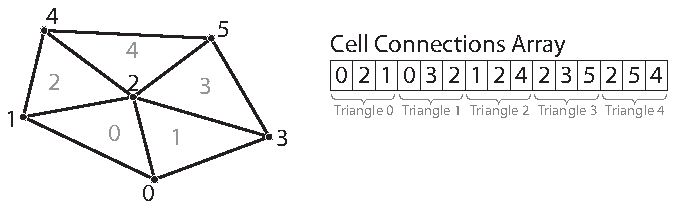
\includegraphics{images/ExplicitCellConnections}
  \caption{An example explicit mesh.}
  \label{fig:ExplicitMesh}
\end{figure}

The \vtkmcont{DataSetBuilderExplicit} class can be used to create data sets
with explicit meshes. \textidentifier{DataSetBuilderExplicit} has several
versions of a method named \textcode{Create}. Generally, these methods take
the shapes, number of indices, and connectivity arrays as well as an array
of point coordinates. These arrays can be given in \textcode{std::vector}
objects, and the data are copied into the \textidentifier{DataSet} created.

The following example creates a mesh like the one shown in
Figure~\ref{fig:ExplicitMesh}.

\vtkmlisting{Creating an explicit mesh with \textidentifier{DataSetBuilderExplicit}.}{CreateExplicitGrid.cxx}

Often it is awkward to build your own arrays and then pass them to
\textidentifier{DataSetBuilderExplicit}. There also exists an alternate
builder class named \vtkmcont{DataSetBuilderExplicitIterative} that allows
you to specify each cell and point one at a time rather than all at once.
This is done by calling one of the versions of \textcode{AddPoint} and one
of the versions of \textcode{AddCell} for each point and cell,
respectively. The next example also builds the mesh shown in
Figure~\ref{fig:ExplicitMesh} except this time using
\textidentifier{DataSetBuilderExplicitIterative}.

\vtkmlisting{Creating an explicit mesh with \textidentifier{DataSetBuilderExplicitIterative}.}{CreateExplicitGridIterative.cxx}

\subsubsection{Add Fields}

In addition to creating the geometric structure of a data set, it is
usually important to add fields to the data. Fields describe numerical data
associated with the topological elements in a cell. They often represent a
physical quantity (such as temperature, mass, or volume fraction) but can
also represent other information (such as indices or classifications).

The easiest way to define fields in a data set is to use the
\vtkmcont{DataSetFieldAdd} class. This class works on
\textidentifier{DataSet}s of any type. It has methods named
\textcode{AddPointField} and \textcode{AddCellField} that define a field
for either points or cells. Every field must have an associated field name.

Both \textcode{AddPointField} and \textcode{AddCellField} are overloaded to
accept arrays of data in different structures. Field arrays can be passed
as standard C arrays or as \textcode{std::vector}s, in which case the data
are copied. Field arrays can also be passed in a
\textidentifier{ArrayHandle}, in which case the data are not copied.

The following (somewhat contrived) example defines fields for a uniform
grid that identify which points and cells are on the boundary of the mesh.

\vtkmlisting{Adding fields to a \textidentifier{DataSet}.}{AddFieldData.cxx}

\index{data~set!Building|)}

\subsection{Cell Sets}
\label{sec:DataSets:CellSets}

\index{cell~set|(}
\index{data~set!cell~set|see{cell~set}}

A cell set determines the topological structure of the data in a data set.
Fundamentally, any cell set is a collection of cells, which typically (but
not always) represent some region in space. 3D cells are made up of points,
edges, and faces. (2D cells have only points and edges, and 1D cells have
only points.) The arrangement of these points, edges, and faces is defined
by the \index{shape}\index{cell~set!shape}\index{cell~shape}\keyterm{shape}
of the cell, which prescribes a specific ordering of each. The basic cell
shapes provided by VTK-m are discussed in detail in
Section~\ref{sec:CellShapeTagsIds} starting on
page~\pageref{sec:CellShapeTagsIds}.

There are multiple ways to express the connections of a cell set, each with
different benefits and restrictions. These different cell set types are
managed by different cell set classes in VTK-m. All VTK-m cell set classes
inherit from \vtkmcont{CellSet}. The two basic types of cell sets are
structured and explicit, and there are several variations of these types.

\subsubsection{Structured Cell Sets}

\index{cell~set!structured|(}
\index{structured~cell~set|(}

A \vtkmcont{CellSetStructured} defines a 1-, 2-, or 3-dimensional grid of
points with lines, quadrilaterals, or hexahedra, respectively, connecting
them. The topology of a \textidentifier{CellSetStructured} is specified by
simply providing the dimensions, which is the number of points in the $i$,
$j$, and $k$ directions of the grid of points. The number of points is
implicitly $i \times j \times k$ and the number of cells is implicitly
$(i-1) \times (j-1) \times (k-1)$ (for 3D grids).
Figure~\ref{fig:CellSetStructured} demonstrates this arrangement.

\begin{figure}
  \centering
  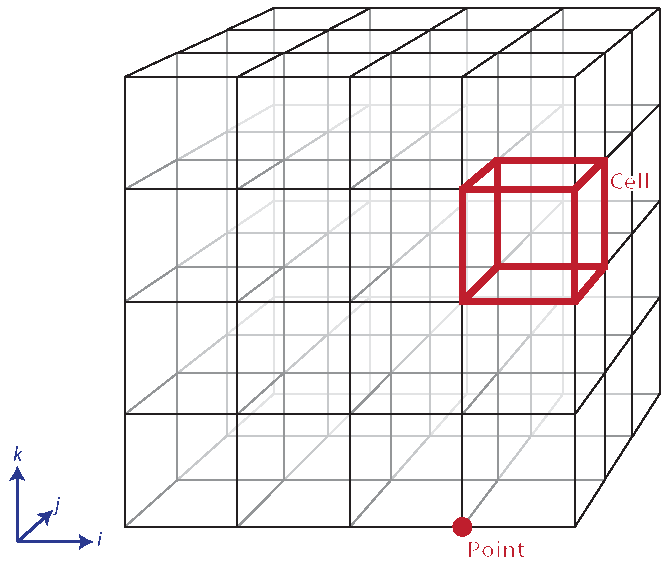
\includegraphics{images/StructuredCellSet}
  \caption{The arrangement of points and cells in a 3D structured grid.}
  \label{fig:CellSetStructured}
\end{figure}

The big advantage of using \vtkmcont{CellSetStructured} to define a cell
set is that it is very space efficient because the entire topology can be
defined by the three integers specifying the dimensions. Also algorithms
can be optimized for \textidentifier{CellSetStructured}'s regular nature.
However, \textidentifier{CellSetStructured}'s strictly regular grid
structure also limits its applicability. A structured cell set can only be
a dense grid of lines, quadrilaterals, or hexahedra. It cannot represent
irregular data well.

Many data models in other software packages, such as the one for VTK, make
a distinction between uniform, rectilinear, and curvilinear grids. VTK-m's
cell sets do not. All three of these grid types are represented by
\textidentifier{CellSetStructured}. This is because in a VTK-m data set the
cell set and the coordinate system are defined independently and used
interchangeably. A structured cell set with uniform point coordinates makes
a uniform grid. A structured cell set with point coordinates defined
irregularly along coordinate axes makes a rectilinear grid. And a
structured cell set with arbitrary point coordinates makes a curvilinear
grid. The point coordinates are defined by the data set's coordinate system,
which is discussed in Section~\ref{sec:DataSets:CoordinateSystems} starting
on page~\pageref{sec:DataSets:CoordinateSystems}.

\index{structured~cell~set|)}
\index{cell~set!structured|)}

\subsubsection{Explicit Cell Sets}

\index{explicit~cell~set|(}
\index{cell~set!explicit|(}

A \vtkmcont{CellSetExplicit} defines an irregular collection of cells. The
cells can be of different types and connected in arbitrary ways. This is
done by explicitly providing for each cell a sequence of points that
defines the cell.

An explicit cell set is defined with a minimum of three arrays. The first
array identifies the shape of each cell. (Cell shapes are discussed in
detail in Section~\ref{sec:CellShapeTagsIds} starting on
page~\pageref{sec:CellShapeTagsIds}.) The second array identifies how many
points are in each cell. The third array has a sequence of point indices
that make up each cell. Figure~\ref{fig:CellSetExplicit} shows a simple
example of an explicit cell set.

\begin{figure}
  \centering
  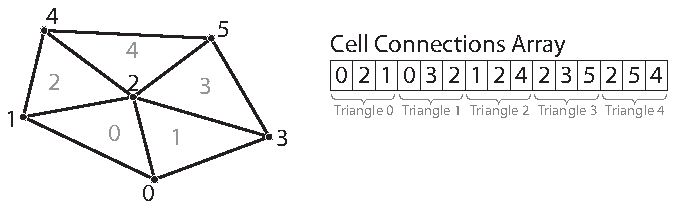
\includegraphics{images/ExplicitCellConnections}
  \caption{Example of cells in a \textidentifier{CellSetExplict} and the
    arrays that define them.}
  \label{fig:CellSetExplicit}
\end{figure}

An explicit cell set may also have other topological arrays such as an
array of offsets of each cell into the connectivity array or an array of
cells incident on each point. Although these arrays can be provided, they
are optional and can be internally derived from the shape, num indices, and
connectivity arrays.

\vtkmcont{ExplicitCellSet} is a powerful representation for a cell set
because it can represent an arbitrary collection of cells. However, because
all connections must be explicitly defined,
\textidentifier{ExplicitCellSet} requires a significant amount of memory to
represent the topology.

\index{cell~set!single~type|(}
\index{explicit~cell~set!single~type|(}
\index{single~type~cell~set|(}

An important specialization of an explicit cell set is
\vtkmcont{CellSetSingleType}. \textidentifier{CellSetSingleType} is an
explicit cell set constrained to contain cells that all have the same shape
and all have the same number of points. So for example if you are creating
a surface that you know will contain only triangles,
\textidentifier{CellSetSingleType} is a good representation for these data.

Using \textidentifier{CellSetSingleType} saves memory because the array of
cell shapes and the array of point counts no longer need to be stored.
\textidentifier{CellSetSingleType} also allows VTK-m to skip some
processing and other storage required for general explicit cell sets.

\index{single~type~cell~set|)}
\index{explicit~cell~set!single~type|)}
\index{cell~set!single~type|)}

\index{cell~set!explicit|)}
\index{explicit~cell~set|)}

\subsubsection{Cell Set Permutations}

\index{permutation~cell~set|(}
\index{cell~set!permutation|(}

A \vtkmcont{CellSetPermutation} rearranges the cells of one cell set to
create another cell set. This restructuring of cells is not done by copying
data to a new structure. Rather, \textidentifier{CellSetPermutation}
establishes a look-up from one cell structure to another. Cells are permuted
on the fly while algorithms are run.

A \textidentifier{CellSetPermutation} is established by providing a mapping
array that for every cell index provides the equivalent cell index in the
cell set being permuted. \textidentifier{CellSetPermutation} is most often
used to mask out cells in a data set so that algorithms will skip over
those cells when running. Note that although
\textidentifier{CellSetPermutation} can mask cells, it cannot mask points.
All points from the original cell set are available in the permuted cell
set regardless of whether they are used.

The following example uses \vtkmcont{CellSetPermutation} with a counting
array to expose every tenth cell. This provides a simple way to subsample a
data set.

\vtkmlisting{Subsampling a data set with \textidentifier{CellSetPermutation}.}{CreateCellSetPermutation.cxx}

\index{cell~set!permutation|)}
\index{permutation~cell~set|)}

\subsubsection{Dynamic Cell Sets}

\index{dynamic~cell~set|(}
\index{cell~set!dynamic|(}

\vtkmcont{DataSet} must hold an arbitrary collection of \vtkmcont{CellSet}
objects, which it cannot do while knowing their types at compile time. To
manage storing \textidentifier{CellSet}s without knowing their types,
\textidentifier{DataSet} actually holds references using
\vtkmcont{DynamicCellSet}.

\textidentifier{DynamicCellSet} is similar in nature to
\textidentifier{DynamicArrayHandle} except that it, of course, holds
\textidentifier{CellSet}s instead of \textidentifier{ArrayHandle}s. The
interface for the two classes is similar, and you should review the
documentation for \textidentifier{DynamicArrayHandle} (in
Section~\ref{sec:DynamicArrayHandle} starting on
page~\pageref{sec:DynamicArrayHandle}) to understand
\textidentifier{DynamicCellSet}.

\vtkmcont{DynamicCellSet} has a method named \textcode{GetCellSet} that
returns a const reference to the held cell set as the abstract
\textidentifier{CellSet} class. This can be used to easily access the
virtual methods in the \textidentifier{CellSet} interface. You can also
create a new instance of a cell set with the same type using the
\textcode{NewInstance} method.

The \textidentifier{DynamicCellSet}\textcode{::IsType()} method can be used
to determine whether the cell set held in the dynamic cell set is of a
given type. If the cell set type is known,
\textidentifier{DynamicCellSet}\textcode{::CastTo()} can be used to safely
downcast the cell set object.

When a typed version of the cell set stored in the
\textidentifier{DynamicCellSet} is needed but the type is not known, which
happens regularly in the internal workings of VTK-m, the
\textcode{CastAndCall} method can be used to make this transition.
\textcode{CastAndCall} works by taking a functor and calls it with the
appropriately cast cell set object.

The \textcode{CastAndCall} method works by attempting to cast to a known
set of types. This set of types used is defined by the macro
\vtkmmacro{VTKM\_DEFAULT\_CELL\_SET\_LIST\_TAG}, which is declared in
\vtkmheader{vtkm/cont}{CellSetListTag.h}. This list can be overridden
globally by defining the \vtkmmacro{VTKM\_DEFAULT\_CELL\_SET\_LIST\_TAG}
macro \emph{before} any VTK-m headers are included.

The set of types used in a \textcode{CastAndCall} can also be changed only
for a particular instance of a dynamic cell set by calling its
\textcode{ResetCellSetList}. This method takes a list of cell types and
returns a new dynamic array handle of a slightly different type that will
use this new list of cells for dynamic casting.

\index{cell~set!dynamic|)}
\index{dynamic~cell~set|}

\subsubsection{Blocks and Assemblies}

Rather than just one cell set, a \vtkmcont{DataSet} can hold multiple cell
sets. This can be used to construct multiblock data structures or
assemblies of parts. Multiple cell sets can also be used to represent
subsets of the data with particular properties such as all cells filled
with a material of a certain type. Or these multiple cells might represent
particular features in the data, such as the set of faces representing a
boundary in the simulation.

\subsubsection{Zero Cell Sets}

It is also possible to construct a \vtkmcont{DataSet} that contains no cell
set objects whatsoever. This can be used to manage data that does not
contain any topological structure. For example, a collection of series that
come from columns in a table could be stored as multiple fields in a data
set with no cell set.

\index{cell~set|)}

\subsection{Fields}
\label{sec:DataSets:Fields}

\index{field|(}
\index{data~set!field|see{field}}

A field on a data set provides a value on every point in space on the mesh.
Fields are often used to describe physical properties such as pressure,
temperature, mass, velocity, and much more. Fields are represented in a
VTK-m data set as an array where each value is associated with a particular
element type of a mesh (such as points or cells). This association of field
values to mesh elements and the structure of the cell set determines how
the field is interpolated throughout the space of the mesh.

Fields are manged by the \vtkmcont{Field} class. \textidentifier{Field}
holds its data with a \textidentifier{DynamicArrayHandle}, which itself is
a container for an \textidentifier{ArrayHandle}. \textidentifier{Field}
also maintains the association and, optionally, the name of a cell set for
which the field is valid.

The data array can be retrieved as a \textidentifier{DynamicArrayHandle}
using the \textcode{GetData} method of \textidentifier{Field}.
\textidentifier{Field} also has a convenience method named
\textcode{GetBounds} that finds the range of values stored in the field
array.

\index{field|}

\subsection{Coordinate Systems}
\label{sec:DataSets:CoordinateSystems}

\index{coordinate~system|(}
\index{data~set!coordinate~system|see{coordinate~system}}

A coordinate system determines the location of a mesh's elements in space.
The spatial location is described by providing a 3D vector at each point
that gives the coordinates there. The point coordinates can then be
interpolated throughout the mesh.

Coordinate systems are managed by the \vtkmcont{CoordinateSystem} class. In
actuality, a coordinate system is just a field with a special meaning, and
so the \textidentifier{CoordinateSystem} class inherits from the
\textidentifier{Field} class. \textidentifier{CoordinateSystem} constrains
the field to be associated with points and typically has 3D floating point
vectors for values.

It is typical for a \textidentifier{DataSet} to have one coordinate system
defined, but it is possible to define multiple coordinate systems. This is
helpful when there are multiple ways to express coordinates. For example,
positions in geographic may be expressed as Cartesian coordinates or as
latitude-longitude coordinates. Both are valid and useful in different
ways.

It is also valid to have a \textidentifier{DataSet} with no coordinate
system. This is useful when the structure is not rooted in physical space.
For example, if the cell set is representing a graph structure, there might
not be any physical space that has meaning for the graph.

\index{coordinate~system|)}

\index{data~set|)}

%% The Dax toolkit provides containers for topologies. The topologies are
%% built on the previously described data structures (mostly array handles)
%% and are intentionally simplistic to simplify the adaptation to other
%% structures.

%% The grid structures are independent classes. They have no common
%% superclass. However, they do have some elements that are expected to be
%% common across all grids classes, which can be used in a templated
%% environment.

%% All grid structures have methods named \index{GetNumberOfPoints}
%% \textcode{GetNumberOfPoints} and \index{GetNumberOfCells}
%% \textcode{GetNumberOfCells}. These methods, of course, return the number of
%% points or cells in the grid structure.

%% \index{GetPointCoordiantes} All grid structures have a method called
%% \textcode{GetPointCoordinates}. This method returns an array handle that
%% contains the spatial coordinates for all the points in the mesh. Topologies
%% with implicit connections might return an array with an implicit or derived
%% container (meaning that the data is functionally defined rather than stored
%% in memory), but the arrays behave the same regardless. The type of the
%% array returned by \textcode{GetPointCoordinates} is specified by the type
%% \textcode{PointCoordinatesType} defined in the grid class. This will be
%% either a \textcode{typedef} of an \textidentifier{ArrayHandle} with
%% specific template parameters or a subclass of
%% \textidentifier{ArrayHandle}.

%% \index{ComputePointCoordinates} It is also possible to query the point
%% coordinates for any given point with the \textcode{ComputePointCoordinates}
%% method. This method is mainly provided for testing purposes. Most point
%% coordinate operations should be performed in the execution environment.

%% The \textcode{GetPointCoordinates} method is most useful for invoking an
%% operation on the point coordinates as a field on points. We have seen this
%% method used on the examples of the elevation worklet.

%% \begin{daxexample}{Processing point coordinates from an unknown grid type.}
%% template<typename GridType>
%% DAX_CONT_EXPORT
%% void Elevation(const GridType &grid,
%%                dax::cont::ArrayHandle<dax::Scalar> &outPointElevation)
%% {
%%   dax::cont::DispatcherMapField<dax::worklet::Elevation> dispatcher;
%%   dispatcher.Invoke(grid.GetPointCoordinates(), outPointElevation);
%% }
%% \end{daxexample}

%% Each grid structure contains a particular type of cell. Each grid structure
%% defines a type named \index{CellTag} \textcode{CellTag} that identifies the
%% type of cell stored. Cell types and operations that can be performed in the
%% execution environment are described in
%% Section~\ref{sec:CellsAndOperations}.

%% All grid structures also have the facilities to pack information to be sent
%% to the execution environment. There is a type defined in the grid class
%% called \textcode{TopologyStructConstExecution} for read-only input data and
%% a \textcode{PrepareForInput} method to build the structure. Likewise, there
%% is a \textcode{TopologyStructExecution} type and
%% \textcode{PrepareForOutput} method for output data.

%% The execution structures, however, differ significantly. Typically, these
%% facilities are handled internally within Dax to pass data to worklets.

%% \subsection{Uniform Grid}

%% \index{uniform~grid|(}

%% A uniform grid is stored in a \daxcont{UniformGrid} class. A uniform grid
%% is a topology structure where its points form a regular 3D array. The 3D
%% array of points are axis aligned, and the spacing is uniform along each
%% dimension. Adjacent are connected together in \index{voxel} \keyterm{voxel}
%% cells, which are simply axis aligned hexahedra.

%% The topology of a uniform grid is completely implicit and specified with
%% three pieces of information. First, the extent, stored in a \dax{Extent3}
%% structure, specifies the minimum and maximum indices of the array. Second,
%% the origin, stored in a \dax{Vector3}, gives the point coordinates of the
%% point at index $[0,0,0]$ (which may not actually be in the extent of the
%% grid). Third, the spacing, stored in a \dax{Vector3}, gives the amount of
%% space between adjacent points in each dimension.

%% The uniform grid class is templated on the device adapter for which it is
%% being used. Its prototype looks as follows.

%% \begin{daxexample}{Prototype for \protect\daxcont{UniformGrid}.}
%% template <class DeviceAdapterTag = DAX_DEFAULT_DEVICE_ADAPTER_TAG>
%% class UniformGrid;
%% \end{daxexample}

%% The \daxcont{UniformGrid} class provides the following features.
%% \begin{description}
%% \item[\textcode{CellTag}] A type that identifies what kind of cell is
%%   stored in this class. Always set to \dax{CellTagVoxel}.
%% \item[\textcode{GetExtent}] A method that returns a \dax{Extent3}
%%   specifying the extent of the 3 dimensional indices.
%% \item[\textcode{SetExtent}] A method that sets the extent of the 3
%%   dimensional indices. There are two versions of \textcode{SetExtent}: one
%%   that accepts a \dax{Extent3} object and another that accepts two
%%   \dax{Id3} objects specifying the minimum and maximum indices.
%% \item[\textcode{GetOrigin}] A method that returns a \dax{Vector3}
%%   specifying the coordinates for the origin of the grid.
%% \item[\textcode{SetOrigin}] A method that accepts a \dax{Vector3} as a
%%   parameter to set the coordinates for the origin of the grid.
%% \item[\textcode{GetSpacing}] A method that returns a \dax{Vector3}
%%   specifying the spacing between adjacent points along each dimension.
%% \item[\textcode{SetSpacing}] A method that accepts a \dax{Vector3} as a
%%   parameter to set the spacing between adjacent points along each
%%   dimension.
%% \item[\textcode{GetNumberOfPoints}] A method that returns the number of
%%   points in the grid.
%% \item[\textcode{GetNumberOfCells}] A method that returns the number of
%%   cells in the grid.
%% \item[\textcode{ComputePointIndex}] A convenience method that takes a
%%   \dax{Id3} representing the 3 dimensional coordinates of a point and
%%   returns the one dimensional index for the point. The 1 dimensional index
%%   corresponds to the index for point field arrays contained in
%%   \daxcont{ArrayHandle} objects.
%% \item[\textcode{ComputeCellIndex}] A convenience method that takes a
%%   \dax{Id3} representing the 3 dimensional coordinates of a cell and
%%   returns the one dimensional index for the cell. The 1 dimensional index
%%   corresponds to the index for cell field arrays contained in
%%   \daxcont{ArrayHandle} objects.
%% \item[\textcode{ComputePointLocation}] A convenience method that takes a 1
%%   dimensional point index and returns the corresponding 3 dimensional index
%%   as a \dax{Id3}. This method performs the inverse operation of
%%   \textcode{ComputePointIndex}.
%% \item[\textcode{ComputeCellLocation}] A convenience method that takes a 1
%%   dimensional cell index and returns the corresponding 3 dimensional index
%%   as a \dax{Id3}. This method performs the inverse operation of
%%   \textcode{ComputeCellIndex}.
%% \item[\textcode{ComputePointCoordinates}] A convenience method that
%%   returns the spatial coordinates for a given point. This method is
%%   overloaded to accept either a 1 dimensional index as a \dax{Id} or a 3
%%   dimensional index as a \dax{Id3}.
%% \item[\textcode{GetPointCoordinates}] Returns a \daxcont{ArrayHandle}
%%   containing spatial coordinates for each point. This array can be used as
%%   a field when invoking worklets. The array is implicit.
%% \item[\textcode{PointCoordinatesType}] The type returned by
%%   \textcode{GetPointCoordinates}. It is a specialization of
%%   \textidentifier{ArrayHandle}.
%% \item[\textcode{TopologyStructConstExecution}] A memory copyable structure
%%   holding the state of the uniform grid that can be used in the execution
%%   environment.
%% \item[\textcode{PrepareForInput}] A method that returns a
%%   \textcode{TopologyStructConstExecution} object to pass to the execution
%%   environment. This method is typically only used internally within the Dax
%%   toolkit.
%% \end{description}

%% \index{uniform~grid|)}

%% \subsection{Unstructured Grid}

%% \index{unstructured~grid|(}

%% An unstructured grid is stored in a \daxcont{UnstructuredGrid} class. An
%% unstructured grid is a topology with a collection of cells connected in
%% arbitrary ways. It first defines a list of points. It then has a connection
%% list that specifies for each cell the points that comprise the vertices for
%% each cell. The \daxcont{UnstructuredGrid} class is limited to containing
%% cells of only one type.

%% The topology of an unstructured grid is defined with a point coordinates
%% array and a cell connections array. The point coordinates array is an array
%% of \dax{Vertex3} values containing one for each point. The cell connections
%% array is an array of \dax{Id} values. The length of this array is the
%% number of cells times the number of vertices per cell. The connections for
%% a particular cell are grouped together in adjacent array values. The cell
%% connections are given in CGNS order\lcite{CGNS}. An example cell connection
%% array is given in Figure~\ref{fig:CellConnections}.

%% \begin{figure}[htb]
%%   \centering
%%   \includegraphics{images/CellConnections}
%%   \caption{The cell connection array for a simple triangle mesh.}
%%   \label{fig:CellConnections}
%% \end{figure}

%% The unstructured grid class is templated on the cell type
%% (\dax{CellTagHexahedron}, \dax{CellTagLine}, \dax{CellTagQuadrilateral},
%% \dax{CellTagTetrahedron}, \dax{CellTagTriangle}, \dax{CellTagVertex}, or
%% \dax{CellTagWedge}) the container for cell connections, the container for
%% the point coordinate array, and the device adapter. Its prototype looks as
%% follows.

%% \begin{daxexample}{Prototype for \protect\daxcont{UnstructuredGrid}.}
%% template <
%%     typename CellT,
%%     class CellConnectionsContainerControlTag = DAX_DEFAULT_ARRAY_CONTAINER_CONTROL_TAG,
%%     class PointsArrayContainerControlTag = DAX_DEFAULT_ARRAY_CONTAINER_CONTROL_TAG,
%%     class DeviceAdapterTag = DAX_DEFAULT_DEVICE_ADAPTER_TAG>
%% class UnstructuredGrid;
%% \end{daxexample}

%% The \daxcont{UnstructuredGrid} class provides the following features.
%% \begin{description}
%% \item[\textcode{CellTag}] A type that identifies what kind of cell is
%%   stored in this class. Always set to the first template parameter.
%% \item[\textcode{CellConnectionsType}] The type of the \daxcont{ArrayHandle}
%%   used to store cell connection indices.
%% \item[\textcode{PointCoordinatesType}] The type of the
%%   \daxcont{ArrayHandle} used to store point coordinates.
%% \item[\textcode{GetCellConnections}] A method used to get the array handle
%%   for the cell connections.
%% \item[\textcode{SetCellConnetions}] A method used to set the array handle
%%   for the cell connections.
%% \item[\textcode{GetPointCoordinates}] A method used to get the array handle
%%   for point coordinates.
%% \item[\textcode{SetPointCoordinates}] A method used to set the array handle
%%   for point coordinates.
%% \item[\textcode{ComputePointCoordinates}] A convenience method that takes a
%%   point index and returns the point coordinates at that index. The actual
%%   value is pulled from the point coordinates array.
%% \item[\textcode{GetNumberOfPoints}] A method that returns the number of
%%   points in the grid.
%% \item[\textcode{GetNumberOfCells}] A method that returns the number of
%%   cells in the grid.
%% \item[\textcode{TopologyStructExecution}] A memory copyable structure
%%   holding the state of the uniform grid that can be used in the execution
%%   environment.
%% \item[\textcode{TopologyStructConstExecution}] A read-only (const) form of
%%   \textcode{TopologyStructuExecution}.
%% \item[\textcode{PrepareForInput}] A method that returns a
%%   \textcode{TopologyStructConstExecution} object to pass to the execution
%%   environment. This method is typically only used internally within the Dax
%%   toolkit.
%% \item[\textcode{PrepareForOutput}] A method that returns a
%%   \textcode{TopologyStructExecution} object to pass to the execution
%%   environment. This method is typically only used internally within the Dax
%%   toolkit.
%% \end{description}

%% \index{unstructured~grid|)}

\section{Timers}
\label{sec:Timers}

\index{timer|(}

It is often the case that you need to measure the time it takes for an
operation to happen. This could be for performing measurements for
algorithm study or it could be to dynamically adjust scheduling.

Performing timing in a multi-threaded environment can be tricky because
operations happen asynchronously. In the VTK-m control environment timing
is simplified because the control environment operates on a single
thread. However, operations invoked in the execution environment may run
asynchronously to operations in the control environment.

To ensure that accurate timings can be made, VTK-m provides a
\vtkmcont{Timer} class that is templated on the device adapter to provide
an accurate measurement of operations that happen on the device. If not
template parameter is provided, the default device adapter is used.

The timing starts when the \textidentifier{Timer} is constructed. The time
elapsed can be retrieved with a call to the \textcode{GetElapsedTime}
method. This method will block until all operations in the execution
environment complete so as to return an accurate time. The timer can be
restarted with a call to the \textcode{Reset} method.

\fix{This example needs to be updated when something interesting can be
  invoked.}

\vtkmlisting{Using \protect\vtkmcont{Timer}.}{Timer.cxx}

\index{timer|)}

\section{Error Handling}
\label{sec:ErrorHandlingControl}

\index{errors|(}

VTK-m uses exceptions to report errors. All exceptions thrown by VTK-m will
be a subclass of \vtkmcont{Error}. For simple error reporting, it is
possible to simply catch a \vtkmcont{Error} and report the error message
string reported by the \textcode{GetMessage} method.

\vtkmlisting{Simple error reporting.}{CatchingErrors.cxx}

There are two subclasses to \vtkmcont{Error}. These are
\vtkmcont{ErrorExecution} and \vtkmcont{ErrorControl}, and they represent
errors that happen in the respective execution and control environments.

\index{errors!execution~environment}
Readers familiar with parallel programming will probably note the
difficulty in raising errors in multi-threaded execution like what happens
in the execution environment. In fact some devices, like CUDA devices, do
not support exceptions at all. VTK-m handles the error reporting in the
execution environment by flagging an error when it occurs and then throwing
an error in the control environment after all threads have terminated. This
means that the amount of execution that happens after an error is flagged
is indeterminate and any output values should be considered incorrect.

The \vtkmcont{ErrorControl} class is also broken down into several
subclasses that can be independently caught to handle different types of
errors. The following control errors exist and may be thrown.
\begin{description}
\item[\vtkmcont{ErrorControlAssert}] \index{assert} \index{errors!assert}
  Thrown when an assertion fails, meaning a VTK-m operation reached an
  unexpected state. The header file \vtkmheader{vtkm/cont}{Assert.h}
  defines a macro named \vtkmmacro{VTKM\_ASSERT\_CONT} that behaves much
  like the POSIX C assert macro except that a
  \textidentifier{ErrorControlAssert} is thrown rather than killing the
  application outright.
\item[\vtkmcont{ErrorControlBadValue}] Thrown when a VTK-m function or
  method encounters an invalid value that inhibits progress.
\item[\vtkmcont{ErrorControlInternal}] Thrown when VTK-m detects an
  internal state that should never be reached. This error usually indicates
  a bug in VTK-m or, at best, VTK-m failed to detect an invalid input it
  should have.
\item[\vtkmcont{ErrorControlOutOfMemory}] Thrown when a VTK-m function or
  method tries to allocate an array and fails.
\end{description}

\index{errors|)}

\index{device~adapter|(}

\section{Device Adapter Algorithms}
\label{sec:DeviceAdapterAlgorithms}

\index{device~adapter!algorithm|(}
\index{algorithm|(}

VTK-m comes with the templated class \vtkmcont{DeviceAdapterAlgorithm} that
provides a set of algorithms that can be invoked in the control environment
and are run on the execution environment. The template has a single
argument that specifies the device adapter tag.

\vtkmlisting{Prototype for \protect\vtkmcont{DeviceAdapterAlgorithm}.}{DeviceAdapterAlgorithmPrototype.cxx}

\textidentifier{DeviceAdapterAlgorithm} contains no state. It only has a
set of static methods that implement its algorithms. The following methods
are available.

\begin{description}
\item[\textcode{Copy}] \index{copy} Copies data from an input array to an
  output array. The copy takes place in the execution environment.
\item[\textcode{LowerBounds}] \index{lower~bounds} The
  \textcode{LowerBounds} method takes three arguments. The first argument
  is an \textidentifier{ArrayHandle} of sorted values. The second argument
  is another \textidentifier{ArrayHandle} of items to find in the first
  array. \textcode{LowerBounds} find the index of the first item that is
  greater than or equal to the target value, much like the
  \textcode{std::lower\_bound} STL algorithm. The results are returned in
  an \textidentifier{ArrayHandle} given in the third argument.

  There are two specializations of \textcode{LowerBounds}. The first takes
  an additional comparison function that defines the less-than
  operation. The second takes only two parameters. The first is an
  \textidentifier{ArrayHandle} of sorted \vtkm{Id}s and the second is an
  \textidentifier{ArrayHandle} of \vtkm{Id}s to find in the first list. The
  results are written back out to the second array. This second
  specialization is useful for inverting index maps.
\item[\textcode{ScanInclusive}] \index{scan!inclusive} The
  \textcode{ScanInclusive} method takes an input and an output
  \textidentifier{ArrayHandle} and performs a running sum on the input
  array. The first value in the output is the same as the first value in
  the input. The second value in the output is the sum of the first two
  values in the input. The third value in the output is the sum of the
  first three values of the input, and so on. \textcode{ScanInclusive}
  returns the sum of all values in the input.
\item[\textcode{ScanExclusive}] \index{scan!exclusive} The
  \textcode{ScanExclusive} method takes an input and an output
  \textidentifier{ArrayHandle} and performs a running sum on the input
  array. The first value in the output is always 0. The second value in the
  output is the same as the first value in the input. The third value in
  the output is the sum of the first two values in the input. The fourth
  value in the output is the sum of the first three values of the input,
  and so on. \textcode{ScanExclusive} returns the sum of all values in the
  input.
\item[\textcode{Schedule}] \index{schedule} The \textcode{Schedule} method
  takes a functor as its first argument and invokes it a number of times
  specified by the second argument. It should be assumed that each
  invocation of the functor occurs on a separate thread although in
  practice there could be some thread sharing.

  There are two versions of the \textcode{Schedule} method. The first
  version takes a \vtkm{Id} and invokes the functor that number of
  times. The second version takes a \vtkm{Id3} and invokes the functor once
  for every entry in a 3D array of the given dimensions.

  The functor is expected to be an object with a const overloaded
  parentheses operator. The operator takes as a parameter the index of the
  invocation, which is either a \vtkm{Id} or a \vtkm{Id3} depending on what
  version of \textcode{Schedule} is being used. The functor must also
  subclass \vtkmexec{FunctorBase}, which provides the error handling
  facilities for the execution environment. \textidentifier{FunctorBase}
  contains a public method named \index{RaiseError}
  \index{errors!execution~environment} \textcode{RaiseError} that takes a
  message and will cause a \vtkmcont{ErrorExecution} exception to be thrown
  in the control environment.
\item[\textcode{Sort}] \index{sort} The \textcode{Sort} method provides an
  unstable sort of an array. There are two forms of the \textcode{Sort}
  method. The first takes an \textidentifier{ArrayHandle} and sorts the
  values in place. The second takes an additional argument that is a
  functor that provides the comparison operation for the sort.
\item[\textcode{SortByKey}] \index{sort!by key} The \textcode{SortByKey}
  method works similarly to the \textcode{Sort} method except that it takes
  two \textidentifier{ArrayHandle}s: an array of keys and a corresponding
  array of values. The sort orders the array of keys in ascending values
  and also reorders the values so they remain paired with the same
  key. Like \textcode{Sort}, \textcode{SortByKey} has a version that sorts
  by the default less-than operator and a version that accepts a custom
  comparison functor.
  \fix{This does not seem to be implemented right now, probably because we
    don't have the zip array handle, but it should be.}
\item[\textcode{StreamCompact}] \index{stream~compact} The
  \textcode{StreamCompact} method selectively removes values from an
  array. The first argument is an \textidentifier{ArrayHandle} to be
  compacted and the second argument is an \textidentifier{ArrayHandle} of
  equal size with flags indicating whether the corresponding input value is
  to be copied to the output. The third argument is an output
  \textidentifier{ArrayHandle} whose length is set to the number of true
  flags in the stencil and the passed values are put in order to the output
  array.

  There is also a second form of \textidentifier{StreamCompact} that only
  has the stencil and output as arguments. In this version, the output gets
  the corresponding index of where the input should be taken from.
\item[\textcode{Synchronize}] \index{synchronize} The
  \textidentifier{Synchronize} method waits for any asynchronous operations
  running on the device to complete and then returns.
\item[\textcode{Unique}] \index{unique} The \textcode{Unique} method
  removes all duplicate values in an \textidentifier{ArrayHandle}. The
  method will only find duplicates if they are adjacent to each other in
  the array. The easiest way to ensure that duplicate values are adjacent
  is to sort the array first.

  There are two versions of \textcode{Unique}. The first uses the equals
  operator to compare entries. The second accepts a binary functor to
  perform the comparisons.
\item[\textcode{UpperBounds}] \index{upper~bounds} The
  \textcode{UpperBounds} method takes three arguments. The first argument
  is an \textidentifier{ArrayHandle} of sorted values. The second argument
  is another \textidentifier{ArrayHandle} of items to find in the first
  array. \textcode{UpperBounds} find the index of the first item that is
  greater than to the target value, much like the
  \textcode{std::upper\_bound} STL algorithm. The results are returned in
  an \textidentifier{ArrayHandle} given in the third argument.

  There are two specializations of \textcode{UpperBounds}. The first takes
  an additional comparison function that defines the less-than
  operation. The second takes only two parameters. The first is an
  \textidentifier{ArrayHandle} of sorted \vtkm{Id}s and the second is an
  \textidentifier{ArrayHandle} of \vtkm{Id}s to find in the first list. The
  results are written back out to the second array. This second
  specialization is useful for inverting index maps.
\end{description}

\index{algorithm|)}
\index{device~adapter!algorithm|)}

%% \section{Implementing Device Adapters}
%% \label{sec:ImplementingDeviceAdapters}

%% The Dax toolkit comes with several implementations of device adapters so
%% that it may be ported to a variety of platforms. It is also possible to
%% provide new device adapters to support yet more devices, compilers, and
%% libraries. A new device adapter provides a tag, a class to manage arrays in
%% the execution environment, a collection of algorithms that run in the
%% execution environment, and (optionally) a timer.

%% Although not strictly necessary, the implementation of device adapters
%% within the Dax toolkit are divided into 3 header files with the names
%% \textfilename{DeviceAdapterTag\textasteriskcentered.h},
%% \textfilename{ArrayManagerExecution\textasteriskcentered.h} and
%% \textfilename{DeviceAdapterAlgorithm\textasteriskcentered.h}. The
%% \textfilename{DeviceAdapter\textasteriskcentered.h} that most code includes
%% is a trivial header that simply includes these other three files. For
%% example, the \daxheader{dax/tbb/cont}{DeviceAdapterTBB.h} for the Intel
%% Threading Building Blocks (TBB) device adapter simply contains the
%% following (with minutia like include guards removed).

%% \begin{daxexample}{Contents of \protect\daxheader{dax/tbb/cont}{DeviceAdapterTBB.h} file.}
%% #include <dax/tbb/cont/internal/DeviceAdapterTagTBB.h>
%% #include <dax/tbb/cont/internal/ArrayManagerExecutionTBB.h>
%% #include <dax/tbb/cont/internal/DeviceAdapterAlgorithmTBB.h>
%% \end{daxexample}

%% The reason the Dax toolkit breaks up the code for its device adapters this
%% way is that there is an interdependence between the implementation of each
%% device adapter and the mechanism to pick a default device adapter. Breaking
%% up the device adapter code in this way maintains an acyclic dependence among
%% header files.

%% \subsection{Tag}

%% The device adapter tag, as described in Section~\ref{sec:DeviceAdapterTag}
%% is a simple empty type that is used as a template parameter to identify the
%% device adapter. Every device adapter implementation provides one. The
%% device adapter tag is typically defined in an internal header file with a
%% prefix of \textfilename{DeviceAdapterTag}. Here is the implementation for
%% the TBB device adapter.

%% \begin{daxexample}{Implementation of the TBB device adapter tag.}
%% namespace dax {
%% namespace tbb {
%% namespace cont {

%% struct DeviceAdapterTagTBB {  };

%% }
%% }
%% } // namespace dax::tbb::cont
%% \end{daxexample}

%% \subsection{Array Manager Execution}

%% \index{device~adapter!array manager|(}
%% \index{array~manager~execution|(}
%% \index{execution~array~manager|(}

%% The Dax toolkit defines a template named
%% \daxcontinternal{ArrayManagerExecution} that is responsible for allocating
%% memory in the execution environment and copying data between the control
%% and execution environment. The execution array manager is typically defined
%% in an internal header file with a prefix of
%% \textfilename{ArrayManagerExecution}.

%% \begin{daxexample}{Prototype for \protect\daxcontinternal{ArrayManagerExecution}.}
%% namespace dax {
%% namespace cont {
%% namespace internal {

%% template<typename T, class ArrayContainerControlTag, class DeviceAdapterTag>
%% class ArrayManagerExecution;

%% }
%% }
%% } // namespace dax::cont::internal
%% \end{daxexample}

%% A device adapter must provide a partial specialization of
%% \textidentifier{ArrayManagerExecution} for its device adapter tag. The
%% implementation for \textidentifier{ArrayManagerExecution} is expected to
%% manage the resources for a single array, and it must provide the following
%% elements.

%% \begin{description}
%% \item[\textcode{ValueType}] A \textcode{typedef} of the type for each item
%%   in the array. This is the same type as the first template argument.
%% \item[\textcode{PortalType}] The type of an array portal that can be used
%%   in the execution environment to access the array.
%% \item[\textcode{PortalConstType}] A read-only (const) version of
%%   \textcode{PortalType}.
%% \item[\textcode{GetNumberOfValues}] A method that returns the number of
%%   values stored in the array. The results are undefined if the data has not
%%   been loaded or allocated.
%% \item[\textcode{LoadDataForInput}] A method that takes an array portal in
%%   the control environment, allocates a large enough array in the execution
%%   environment, and copies the data into that array. The data in the
%%   execution array is not expected to be changed. The allocated array can
%%   later be accessed via the \textcode{GetPortalConst} method.
%% \item[\textcode{LoadDataForInPlace}] A method that takes an array portal in
%%   the control environment, allocates a large enough array in the execution
%%   environment, and copies the data into that array. The data in the
%%   execution array is expected to be read and changed. The allocated array
%%   can later be accessed via the \textcode{GetPortal} and
%%   \textcode{GetPortalConst} methods.
%% \item[\textcode{AllocateArrayForOutput}] A method that takes an array
%%   container and a size and allocates an array in the execution environment
%%   of the specified size. The initial memory is uninitialized and can be
%%   accessed via the \textcode{GetPortal} method. The container argument can
%%   be used to allocate data when the control and execution share arrays, but
%%   this argument is often ignored.
%% \item[\textcode{RetrieveOutputData}] This method takes an array container,
%%   allocates memory in the control environment, and copies data from the
%%   execution environment into it.
%% \item[\textcode{CopyInto}] This method takes an STL-compatible iterator and
%%   copies data from the execution environment into it.
%% \item[\textcode{Shrink}] A method that adjusts the size of the array in the
%%   execution environment to something that is a smaller size. All the data
%%   up to the new length must remain valid. Typically, no memory is actually
%%   reallocated. Instead, a different end is marked.
%% \item[\textcode{GetPortal}] A method that returns an array portal
%%   that can be used in the execution environment. The portal was defined in
%%   either \textcode{LoadDataForInPlace} or
%%   \textcode{AllocateArrayForOutput}.
%% \item[\textcode{GetPortalConst}] A method that returns a read-only
%%   (const) array portal that can be used in the execution environment. The
%%   portal was defined in one of the load or allocate methods.
%% \item[\textcode{ReleaseResources}] A method that frees any resources
%%   (typically memory) in the execution environment.
%% \end{description}

%% Specializations of this template typically take on one of two forms. If the
%% control and execution environments have separate memory spaces, then this
%% class behaves by copying memory in methods such as
%% \textcode{PrepareForInput} and \textcode{RetrieveOutputData}. This might
%% require creating buffers in the control environment to efficiently move
%% data from control array portals.

%% However, if the control and execution environments share the same memory
%% space, the execution array manager can, and should, delegate all of its
%% operations to the \textidentifier{ArrayContainerControl} it is used
%% with. The Dax toolkit comes with a class called
%% \daxcontinternal{ArrayManagerExecutionShareWithControl} that provides the
%% implementation for an execution array manager that shares a memory space
%% with the control environment. In this case, making the
%% \textidentifier{ArrayManagerExecution} specialization be a trivial subclass
%% is sufficient. For example, here is the implementation of
%% \textidentifier{ArrayManagerExecution} for TBB.

%% \begin{daxexample}{Specialization of \textidentifier{ArrayManagerExecution} for TBB.}
%% #include <dax/tbb/cont/internal/DeviceAdapterTagTBB.h>

%% #include <dax/cont/internal/ArrayManagerExecution.h>
%% #include <dax/cont/internal/ArrayManagerExecutionShareWithControl.h>

%% namespace dax {
%% namespace cont {
%% namespace internal {

%% template <typename T, class ArrayContainerTag>
%% class ArrayManagerExecution
%%     <T, ArrayContainerTag, dax::tbb::cont::DeviceAdapterTagTBB>
%%     : public dax::cont::internal::ArrayManagerExecutionShareWithControl
%%         <T, ArrayContainerTag>
%% {
%% };

%% }
%% }
%% } // namespace dax::cont::internal
%% \end{daxexample}

%% \index{execution~array~manager|)}
%% \index{array~manager~execution|)}
%% \index{device~adapter!array manager|)}

%% \subsection{Algorithms}

%% \index{device~adapter!algorithm|(}
%% \index{algorithm|(}

%% A device adapter implementation must also provide a specialization of
%% \daxcont{DeviceAdapterAlgorithm}, which is documented in
%% Section~\ref{sec:DeviceAdapterAlgorithms}. The implementation for the
%% device adapter algorithms is typically placed in a header file with a
%% prefix of \textfilename{DeviceAdapterAlgorithm}.

%% Although there are many methods in
%% \textidentifier{DeviceAdapterAlgorithms}, it is seldom necessary to
%% implement them all. Instead, the Dax toolkit comes with
%% \daxcontinternal{DeviceAdapterAlgorithmGeneral} that provides generic
%% implementation for most of the required algorithms. By deriving the
%% specialization of \textidentifier{DeviceAdapterAlgorithm} from
%% \textidentifier{DeviceAdapterAlgorithmGeneral}, only the implementations
%% for \textcode{Schedule} and \textcode{Synchronize} need to be
%% implemented. All other algorithms can be derived from those.
%% \fix{Document SetErrorMessageBuffer.}

%% That said, not all of the algorithms implemented in
%% \textidentifier{DeviceAdapterAlgorithmGeneral} are optimized for all types
%% of devices. Thus, it is worthwhile to provide algorithms optimized for the
%% specific device when possible. In particular, it is best to provide
%% specializations for the sort and scan algorithms.

%% The following example is a minimal implementation of the TBB device adapter
%% algorithms. The actual version that comes with the Dax toolkit contains
%% more enhancements.

%% \begin{daxexample}{Abbreviated implementation of \textidentifier{DeviceAdapterAlgorithm} for TBB.}
%% #include <dax/tbb/cont/internal/DeviceAdapterTagTBB.h>
%% #include <dax/tbb/cont/internal/ArrayManagerExecutionTBB.h>

%% #include <dax/cont/internal/DeviceAdapterAlgorithmGeneral.h>
%% #include <dax/exec/internal/IJKIndex.h>

%% #include <tbb/blocked_range.h>
%% #include <tbb/blocked_range3d.h>
%% #include <tbb/parallel_for.h>

%% namespace dax {
%% namespace cont {

%% template<>
%% struct DeviceAdapterAlgorithm<dax::tbb::cont::DeviceAdapterTagTBB> :
%%     dax::cont::internal::DeviceAdapterAlgorithmGeneral<
%%         DeviceAdapterAlgorithm<dax::tbb::cont::DeviceAdapterTagTBB>,
%%         dax::tbb::cont::DeviceAdapterTagTBB>
%% {
%% private:
%%   static const dax::Id TBB_GRAIN_SIZE = 128;

%%   template<class FunctorType>
%%   class ScheduleKernel
%%   {
%%   public:
%%     DAX_CONT_EXPORT ScheduleKernel(const FunctorType &functor)
%%       : Functor(functor)
%%     {  }

%%     DAX_CONT_EXPORT void SetErrorMessageBuffer(
%%         const dax::exec::internal::ErrorMessageBuffer &errorMessage)
%%     {
%%       this->ErrorMessage = errorMessage;
%%       this->Functor.SetErrorMessageBuffer(errorMessage);
%%     }

%%     DAX_EXEC_EXPORT
%%     void operator()(const ::tbb::blocked_range<dax::Id> &range) const {
%%       // The TBB device adapter causes array classes to be shared between
%%       // control and execution environment. This means that it is possible for
%%       // an exception to be thrown even though this is typically not allowed.
%%       // Throwing an exception from here is bad because there are several
%%       // simultaneous threads running. Get around the problem by catching the
%%       // error and setting the message buffer as expected.
%%       try
%%         {
%%         for (dax::Id index = range.begin(); index < range.end(); index++)
%%           {
%%           this->Functor(index);
%%           }
%%         }
%%       catch (dax::cont::Error error)
%%         {
%%         this->ErrorMessage.RaiseError(error.GetMessage().c_str());
%%         }
%%       catch (...)
%%         {
%%         this->ErrorMessage.RaiseError(
%%             "Unexpected error in execution environment.");
%%         }
%%     }
%%   private:
%%     FunctorType Functor;
%%     dax::exec::internal::ErrorMessageBuffer ErrorMessage;
%%   };

%% public:
%%   template<class FunctorType>
%%   DAX_CONT_EXPORT
%%   static void Schedule(FunctorType functor, dax::Id numInstances)
%%   {
%%     const dax::Id MESSAGE_SIZE = 1024;
%%     char errorString[MESSAGE_SIZE];
%%     errorString[0] = '\0';
%%     dax::exec::internal::ErrorMessageBuffer
%%         errorMessage(errorString, MESSAGE_SIZE);

%%     ScheduleKernel<FunctorType> kernel(functor);
%%     kernel.SetErrorMessageBuffer(errorMessage);

%%     ::tbb::blocked_range<dax::Id> range(0, numInstances, TBB_GRAIN_SIZE);

%%     ::tbb::parallel_for(range, kernel);

%%     if (errorMessage.IsErrorRaised())
%%       {
%%       throw dax::cont::ErrorExecution(errorString);
%%       }
%%   }

%% private:
%%   template<class FunctorType>
%%   class ScheduleKernelId3
%%   {
%%   public:
%%     DAX_CONT_EXPORT ScheduleKernelId3(const FunctorType &functor,
%%                                       const dax::Id3& dims)
%%       : Functor(functor),
%%         Dims(dims)
%%       {  }

%%     DAX_CONT_EXPORT void SetErrorMessageBuffer(
%%         const dax::exec::internal::ErrorMessageBuffer &errorMessage)
%%     {
%%       this->ErrorMessage = errorMessage;
%%       this->Functor.SetErrorMessageBuffer(errorMessage);
%%     }

%%     DAX_EXEC_EXPORT
%%     void operator()(const ::tbb::blocked_range3d<dax::Id> &range) const {
%%       try
%%         {
%%         dax::exec::internal::IJKIndex index(this->Dims);
%%         for( dax::Id k=range.pages().begin(); k!=range.pages().end(); ++k)
%%           {
%%           index.SetK(k);
%%           for( dax::Id j=range.rows().begin(); j!=range.rows().end(); ++j)
%%             {
%%             index.SetJ(j);
%%             for( dax::Id i=range.cols().begin(); i!=range.cols().end(); ++i)
%%               {
%%               index.SetI(i);
%%               this->Functor(index);
%%               }
%%             }
%%           }
%%         }
%%       catch (dax::cont::Error error)
%%         {
%%         this->ErrorMessage.RaiseError(error.GetMessage().c_str());
%%         }
%%       catch (...)
%%         {
%%         this->ErrorMessage.RaiseError(
%%             "Unexpected error in execution environment.");
%%         }
%%     }
%%   private:
%%     FunctorType Functor;
%%     dax::Id3 Dims;
%%     dax::exec::internal::ErrorMessageBuffer ErrorMessage;
%%   };

%% public:
%%   template<class FunctorType>
%%   DAX_CONT_EXPORT
%%   static void Schedule(FunctorType functor,
%%                        dax::Id3 rangeMax)
%%   {
%%     //we need to extract from the functor that uniform grid information
%%     const dax::Id MESSAGE_SIZE = 1024;
%%     char errorString[MESSAGE_SIZE];
%%     errorString[0] = '\0';
%%     dax::exec::internal::ErrorMessageBuffer
%%         errorMessage(errorString, MESSAGE_SIZE);

%%     //memory is generally setup in a way that iterating the first range
%%     //in the tightest loop has the best cache coherence.
%%     ::tbb::blocked_range3d<dax::Id> range(0, rangeMax[2],
%%                                           0, rangeMax[1],
%%                                           0, rangeMax[0]);

%%     ScheduleKernelId3<FunctorType> kernel(functor,rangeMax);
%%     kernel.SetErrorMessageBuffer(errorMessage);

%%     ::tbb::parallel_for(range, kernel);

%%     if (errorMessage.IsErrorRaised())
%%       {
%%       throw dax::cont::ErrorExecution(errorString);
%%       }
%%   }

%%   DAX_CONT_EXPORT static void Synchronize()
%%   {
%%     // Nothing to do. This device schedules all of its operations using a
%%     // split/join paradigm. This means that the if the control thread is
%%     // calling this method, then nothing should be running in the execution
%%     // environment.
%%   }

%% };

%% }
%% } // namespace dax::cont
%% \end{daxexample}

%% \index{algorithm|)}
%% \index{device~adapter!algorithm|)}

%% \subsection{Timer Implementation}

%% The Dax timer, described in Section~\ref{sec:Timers}, delegates to an
%% internal class named \daxcont{DeviceAdapterTimerImplementation}. The
%% interface for this class is the same as that for \daxcont{Timer}. A default
%% implementation of this templated class uses the system timer and the
%% \textcode{Synchronize} method in the device adapter algorithms.

%% However, some devices might provide alternate or better methods for
%% implementing timers. For example, the TBB library comes with a high
%% resolution timer that has better accuracy than the standard system
%% timers. Thus, the device adapter can optionally provide a specialization of
%% \textidentifier{DeviceAdapterTimerImplementation}, which is typically
%% placed in the same header file as the device adapter algorithms.

%% The following example is the implementation of the TBB timer
%% implementation.

%% \begin{daxexample}{Implementation of \textidentifier{DeviceAdapterTimerImplementation} for TBB.}
%% #include <dax/cont/DeviceAdapter.h>
%% #include <dax/tbb/cont/internal/DeviceAdapterTagTBB.h>

%% #include <tbb/tick_count.h>

%% namespace dax {
%% namespace cont {

%% template<>
%% class DeviceAdapterTimerImplementation<dax::tbb::cont::DeviceAdapterTagTBB>
%% {
%% public:
%%   DAX_CONT_EXPORT DeviceAdapterTimerImplementation()
%%   {
%%     this->Reset();
%%   }
%%   DAX_CONT_EXPORT void Reset()
%%   {
%%     dax::cont::DeviceAdapterAlgorithm<dax::tbb::cont::DeviceAdapterTagTBB>::Synchronize();
%%     this->StartTime = ::tbb::tick_count::now();
%%   }
%%   DAX_CONT_EXPORT dax::Scalar GetElapsedTime()
%%   {
%%     dax::cont::DeviceAdapterAlgorithm<dax::tbb::cont::DeviceAdapterTagTBB>::Synchronize();
%%     ::tbb::tick_count currentTime = ::tbb::tick_count::now();
%%     ::tbb::tick_count::interval_t elapsedTime = currentTime - this->StartTime;
%%     return static_cast<dax::Scalar>(elapsedTime.seconds());
%%   }

%% private:
%%   ::tbb::tick_count StartTime;
%% };

%% }
%% } // namespace dax::cont
%% \end{daxexample}

%% A word of warning about implementing timers. Although
%% \textcode{GetElapsedTime} returns a \dax{Scalar}, it is advisable to store
%% the internal timing in its native data format until the elapsed time is
%% recorded. This is because the times may be biased by a large value, and the
%% floating point number might not hold enough precision to get a precise
%% measurement between the start and end of the timer.

%% \subsection{Testing}

%% The implementation of a device adapter contains many components. To ensure
%% that all of its device adapters are working properly, the Dax toolkit
%% contains a complete test of all the components in
%% \daxheader{dax/cont/testing}{TestingDeviceAdapter.h}. Here is the
%% implementation for the TBB device adapter test, which plugs into the CMake
%% testing framework.

%% \begin{daxexample}{Test code for the TBB device adapter.}
%% #include <dax/tbb/cont/DeviceAdapterTBB.h>

%% #include <dax/cont/testing/TestingDeviceAdapter.h>

%% int UnitTestDeviceAdapterTBB(int, char *[])
%% {
%%   return dax::cont::testing::TestingDeviceAdapter
%%       <dax::tbb::cont::DeviceAdapterTagTBB>::Run();
%% }
%% \end{daxexample}

\index{device~adapter|)}

\index{control~environment|)}

